%% abtex2-modelo-trabalho-academico.tex, v-1.9.6 laurocesar
%% Copyright 2012-2016 by abnTeX2 group at http://www.abntex.net.br/ 
%%
%% This work may be distributed and/or modified under the
%% conditions of the LaTeX Project Public License, either version 1.3
%% of this license or (at your option) any later version.
%% The latest version of this license is in
%%   http://www.latex-project.org/lppl.txt
%% and version 1.3 or later is part of all distributions of LaTeX
%% version 2005/12/01 or later.
%%
%% This work has the LPPL maintenance status `maintained'.
%% 
%% The Current Maintainer of this work is the abnTeX2 team, led
%% by Lauro César Araujo. Further information are available on 
%% http://www.abntex.net.br/
%%
%% This work consists of the files abntex2-modelo-trabalho-academico.tex,
%% abntex2-modelo-include-comandos and abntex2-modelo-references.bib
%%

% ------------------------------------------------------------------------
% ------------------------------------------------------------------------
% abnTeX2: Modelo de Trabalho Academico (tese de doutorado, dissertacao de
% mestrado e trabalhos monograficos em geral) em conformidade com 
% ABNT NBR 14724:2011: Informacao e documentacao - Trabalhos academicos -
% Apresentacao
% ------------------------------------------------------------------------
% ------------------------------------------------------------------------

\documentclass[
	% -- opções da classe memoir --
	12pt,				% tamanho da fonte
	openright,			% capítulos começam em pág ímpar (insere página vazia caso preciso)
	twoside,			% para impressão em recto e verso. Oposto a oneside
	a4paper,			% tamanho do papel. 
	% -- opções da classe abntex2 --
	chapter=TITLE,		% títulos de capítulos convertidos em letras maiúsculas
	%section=TITLE,		% títulos de seções convertidos em letras maiúsculas
	%subsection=TITLE,	% títulos de subseções convertidos em letras maiúsculas
	%subsubsection=TITLE,% títulos de subsubseções convertidos em letras maiúsculas
	% -- opções do pacote babel --
	english,			% idioma adicional para hifenização
	french,				% idioma adicional para hifenização
	spanish,			% idioma adicional para hifenização
	brazil				% o último idioma é o principal do documento
	]{abntex2}

% ---
% Pacotes básicos 
% ---
\usepackage{lmodern}			% Usa a fonte Latin Modern			
\usepackage[T1]{fontenc}		% Selecao de codigos de fonte.
\usepackage[utf8]{inputenc}		% Codificacao do documento (conversão automática dos acentos)
\usepackage{lastpage}			% Usado pela Ficha catalográfica
\usepackage{indentfirst}		% Indenta o primeiro parágrafo de cada seção.
\usepackage{color}				% Controle das cores
\usepackage{graphicx}			% Inclusão de gráficos
\usepackage{microtype} 			% para melhorias de justificação
\usepackage{amsmath}			% para o uso de ferramentas matemáticas
\usepackage{amssymb}
\usepackage{multirow}
\usepackage{subfloat}
\usepackage{pdfpages}


\usepackage{tikz}
\usetikzlibrary{arrows.meta, shapes.geometric}

\settocdepth{subsection}

\tikzset{%
	>={Latex[width=2mm,length=2mm]},
	% Specifications for style of nodes:
	base/.style = {rectangle, rounded corners, draw=black,
		minimum width=5cm, minimum height=1.3cm,
		text centered},
	activityStarts/.style = {base, fill=blue!20},
	decision/.style = { diamond, draw=blue, thick, fill=blue!20, text width=5em, text centered,
		inner sep=3pt, rounded corners },
	startstop/.style = {base, fill=red!30},
	activityRuns/.style = {base, fill=green!30},
	process/.style = {base, minimum width=2.5cm, fill=orange!15},
}

% ---
		
% ---
% Pacotes adicionais, usados apenas no âmbito do Modelo Canônico do abnteX2
% ---
\usepackage{lipsum}				% para geração de dummy text
% ---

% ---
% Pacotes de citações
% ---
\usepackage[brazilian,hyperpageref]{backref}	 % Paginas com as citações na bibl
\usepackage[bibjustif,number]{abntex2cite}	     % Citações padrão ABNT
\citebrackets[]
\usepackage{lscape}

% --- 
% CONFIGURAÇÕES DE PACOTES
% --- 

% ---
% Configurações do pacote backref
% Usado sem a opção hyperpageref de backref
\renewcommand{\backrefpagesname}{Citado na(s) página(s):~}
% Texto padrão antes do número das páginas
\renewcommand{\backref}{}
% Define os textos da citação
\renewcommand*{\backrefalt}[4]{
	\ifcase #1 %
		Nenhuma citação no texto.%
	\or
		Citado na página #2.%
	\else
		Citado #1 vezes nas páginas #2.%
	\fi}%
% ---

% ---
% Informações de dados para CAPA e FOLHA DE ROSTO
% ---
\titulo{Estudo de novos alótropos de carbono por Teoria do Funcional da Densidade}
\autor{Felipe Lopes de Oliveira}
\local{Rio de Janeiro - Brasil}
\data{\today}
\instituicao{%
	Programa de Pós-Graduação em Química
	\par
	Instituto de Química
	\par
	Universidade Federal do Rio de Janeiro - UFRJ}
\tipotrabalho{Dissertação (Mestrado)}
% O preambulo deve conter o tipo do trabalho, o objetivo, 
% o nome da instituição e a área de concentração 
\preambulo{Dissertação de Mestrado apresentada ao Programa de Pós-Graduação em Química (PGQu), do Instituto de Química da Universidade Federal do Rio de Janeiro, como parte dos requisitos necessários à obtenção do título de Mestre em Ciências (Química).}
\orientador{Pierre Mothé Esteves}
\coorientador{Raoni Schroeder Borges Gonçalves}
% ---


% ---
% Configurações de aparência do PDF final

% alterando o aspecto da cor azul
\definecolor{blue}{RGB}{41,5,195}

% informações do PDF
\makeatletter
\hypersetup{
     	%pagebackref=true,
		pdftitle={\@title}, 
		pdfauthor={\@author},
    	pdfsubject={\imprimirpreambulo},
	    pdfcreator={LaTeX with abnTeX2},
		pdfkeywords={abnt}{latex}{abntex}{abntex2}{trabalho acadêmico}, 
		colorlinks=true,       		% false: boxed links; true: colored links
    	linkcolor=black,          	% color of internal links
    	citecolor=black,        		% color of links to bibliography
    	filecolor=black,      		% color of file links
		urlcolor=black,
		bookmarksdepth=4,
		hidelinks
}
\makeatother
% --- 

% --- 
% Espaçamentos entre linhas e parágrafos 
% --- 

% O tamanho do parágrafo é dado por:
\setlength{\parindent}{1.3cm}

% Controle do espaçamento entre um parágrafo e outro:
\setlength{\parskip}{0.2cm}  % tente também \onelineskip

% ---
% compila o indice
% ---
\makeindex
% ---

% ----
% Início do documento
% ----
\begin{document}

\pagenumbering{roman}

% Seleciona o idioma do documento (conforme pacotes do babel)
%\selectlanguage{english}
\selectlanguage{brazil}

% Retira espaço extra obsoleto entre as frases.
\frenchspacing 

% ----------------------------------------------------------
% ELEMENTOS PRÉ-TEXTUAIS
% ----------------------------------------------------------
% \pretextual

% ---
% Capa
% ---
\begin{figure}
	\centering
	\includegraphics[scale=0.35]{capitulos/fig/minerva}
	\label{minerva}
\end{figure}

\textsc{\Large Universidade Federal do Rio de Janeiro} %Major heading such as course name


\imprimircapa
% ---

% ---
% Folha de rosto
% (o * indica que haverá a ficha bibliográfica)
% ---
\imprimirfolhaderosto*
% ---

% ---
% Inserir a ficha bibliografica
% ---

% Isto é um exemplo de Ficha Catalográfica, ou ``Dados internacionais de
% catalogação-na-publicação''. Você pode utilizar este modelo como referência. 
% Porém, provavelmente a biblioteca da sua universidade lhe fornecerá um PDF
% com a ficha catalográfica definitiva após a defesa do trabalho. Quando estiver
% com o documento, salve-o como PDF no diretório do seu projeto e substitua todo
% o conteúdo de implementação deste arquivo pelo comando abaixo:
%
% \begin{fichacatalografica}
%     \includepdf{fig_ficha_catalografica.pdf}
% \end{fichacatalografica}

\begin{fichacatalografica}
	\sffamily
	\vspace*{\fill}					% Posição vertical
	\begin{center}					% Minipage Centralizado
	\fbox{\begin{minipage}[c][8cm]{13.5cm}		% Largura
	\small
	\imprimirautor
	%Sobrenome, Nome do autor
	
	\hspace{0.5cm} \imprimirtitulo  / \imprimirautor. --
	\imprimirlocal, \imprimirdata-
	
	\hspace{0.5cm} \pageref{LastPage} p. : il. (algumas color.) ; 30 cm.\\
	
	\hspace{0.5cm} \imprimirorientadorRotulo~\imprimirorientador
	
	\hspace{0.5cm} \imprimircoorientadorRotulo~\imprimircoorientador\\
	
	\hspace{0.5cm}
	\parbox[t]{\textwidth}{\imprimirtipotrabalho~--~\imprimirinstituicao,
	\imprimirdata.}\\
	
	\hspace{0.5cm}
		1. Carbono.
		2. Alótropos.
		3. Teoria do Funcional da Densidade.
		I. \imprimirorientador . 
		II. \imprimircoorientador . 
		III. Universidade Federal do Rio de Janeiro.
		IV. Instituto de Química, Programa de Pós Graduação em Química
		V. \imprimirtitulo		
	\end{minipage}}
	\end{center}
\end{fichacatalografica}
% ---

% ---
% Inserir errata
% ---
%	\begin{errata}
%	Elemento opcional da \citeonline[4.2.1.2]{NBR14724:2011}. Exemplo:
%	
%	\vspace{\onelineskip}
%	
%	FERRIGNO, C. R. A. \textbf{Tratamento de neoplasias ósseas apendiculares com
%	reimplantação de enxerto ósseo autólogo autoclavado associado ao plasma
%	rico em plaquetas}: estudo crítico na cirurgia de preservação de membro em
%	cães. 2011. 128 f. Tese (Livre-Docência) - Faculdade de Medicina Veterinária e
%	Zootecnia, Universidade de São Paulo, São Paulo, 2011.
%	
%	\begin{table}[htb]
%	\center
%	\footnotesize
%	\begin{tabular}{|p{1.4cm}|p{1cm}|p{3cm}|p{3cm}|}
%	  \hline
%	   \textbf{Folha} & \textbf{Linha}  & \textbf{Onde se lê}  & \textbf{Leia-se}  \\
%	    \hline
%	    1 & 10 & auto-conclavo & autoconclavo\\
%	   \hline
%	\end{tabular}
%	\end{table}
%	
%	\end{errata}
% ---

% ---
% Inserir folha de aprovação
% ---

% Isto é um exemplo de Folha de aprovação, elemento obrigatório da NBR
% 14724/2011 (seção 4.2.1.3). Você pode utilizar este modelo até a aprovação
% do trabalho. Após isso, substitua todo o conteúdo deste arquivo por uma
% imagem da página assinada pela banca com o comando abaixo:
%
% \includepdf{folhadeaprovacao_final.pdf}
%
\begin{folhadeaprovacao}

  \begin{center}
    {\ABNTEXchapterfont\large\imprimirautor}

    \vspace*{\fill}\vspace*{\fill}
    \begin{center}
      \ABNTEXchapterfont\bfseries\Large\imprimirtitulo
    \end{center}
    \vspace*{\fill}
    
    \hspace{.45\textwidth}
    \begin{minipage}{.5\textwidth}
        \imprimirpreambulo
    \end{minipage}%
    \vspace*{\fill}
   \end{center}
        
   Trabalho aprovado. \imprimirlocal, 04 de março de 2020:

   \assinatura{\textbf{Prof. Dr. \imprimirorientador} \\ Presidente e Orientador} 
   %\assinatura{\textbf{Prof. Dr. \imprimircoorientador} \\ Coorientador} 
   %\assinatura{\textbf{Prof. Dr. Rodrigo Barbosa Capaz} \\ IF-UFRJ}
   \assinatura{\textbf{Prof. Dr. Rodrigo José Corrêa} \\ IQ-UFRJ}
   \assinatura{\textbf{Prof. Dr. Itamar Borges Júnior} \\ IME}
   %\assinatura{\textbf{Professor} \\ Convidado 4}
      
   \begin{center}
    \vspace*{0.5cm}
    {\large\imprimirlocal}
    \par
    {\large\imprimirdata}
    \vspace*{1cm}
  \end{center}
  
\end{folhadeaprovacao}
% ---

% ---
% Dedicatória
% ---
\begin{dedicatoria}
   \vspace*{\fill}
   \centering
   \noindent
   \textit{Dedicado a minha família.} \vspace*{\fill}
\end{dedicatoria}
% ---

% ---
% Agradecimentos
% ---
\begin{agradecimentos}
	Primeiramente gostaria de agradecer à minha família, por todo apoio e incentivo dado durante essa jornada. 
	
	
	Aos meu orientador Pierre Mothé Esteves, pelo apoio, amizade e inspiradoras discussões. Ao meu coorientador Raoni Schröeder pelas oportunidades e incentivo. 
	
	Aos amigos do INTERLAB, pela convivência, carinho, amizade e ótimas histórias enquanto tomamos café. 
	A Renata Avena Maia, agora Doutora Maia, pelas longas horas de trabalho que dividimos, pelas muitas colaborações e discussões, pela amizade, por todo o apoio que me deu e por ser modelo de profissional e pessoa a qual me inspirarei na longa jornada que ainda tenho pela frente.
	A Jéssica Bayer, por ter me aturado, motivado, acompanhado durante essa jornada e por ser especial na minha vida. 
	
	Aos professores e amigos do programa de pós-graduação pelas lições ensinadas. Às agências de fomento, CNPq, CAPES e FAPERJ, que mesmo nesse período sombrio pelo qual o país está passando financiaram esse trabalho. Ao NACAD pelos recursos computacionais. Ao Sci-Hub, por fornecer acesso ao conhecimento gerado pela humanidade. 
	
	Por fim, a todos aqueles que mesmo sem saber me influenciaram durante essa jornada. 

\end{agradecimentos}
% ---

% ---
% Epígrafe
% ---
\begin{epigrafe}
    \vspace*{\fill}
	\begin{flushright}
		\textit{Tudo é infinto \\
		no mundo das ideias \\
		não há um fim p'r'o pensar. \\
		Ideias não têm limites \\}
		\end{flushright}

	\begin{flushright}
	\textit{Limites quem têm são pessoas \\
		(as mesmas que têm as ideias) \\
		são elas que lhes dão - às ideias - \\
		um limite, um fim \\
		que é delas - das pessoas -, só delas... só. \\}
	\end{flushright}

	\begin{flushright}
	\textit{Já as coisas da matéria \\
		elas sim, têm sempre um fim.\\
		São limitadas no tempo: \\
		um dia nascem, morrem um dia \\
		todas elas têm um fim. \\
		Também no espaço há limites \\
		que o vazio do entorno \\
		lhes contorna, lhes dá fim. \\}
	\end{flushright}

	\begin{flushright}
	(POETICES - Claudio Costa Neto )
	\end{flushright}
\end{epigrafe}
% ---

% ---
% RESUMOS
% ---

% resumo em português
\setlength{\absparsep}{18pt} % ajusta o espaçamento dos parágrafos do resumo
\begin{resumo}
	
	A vida como conhecemos é totalmente baseada em compostos que são formados estruturalmente por átomos de carbono. A diversidade estrutural resultante dos diferentes tipos de ligações que o carbono pode fazer e sua capacidade de formar ligações químicas fortes e estáveis com outros átomos de carbono resulta em uma miríade de moléculas e materiais. O controle correto dessas ligações resulta em aplicações tecnológicas que vão desde o desenvolvimento de novas moléculas bioativas, como fármacos, até a produção novos materiais sintéticos. 	
	Ao longo da evolução da humanidade, o carbono adquiriu um papel cada vez mais central no desenvolvimento tecnológico. Inicialmente, sua principal utilização era como fonte de energia na forma dos combustíveis como carvão, gás natural e fósseis derivados de petróleo. Entretanto, nas últimas décadas têm havido um crescente interesse em estruturas formadas unicamente por átomos de carbono, denominadas alótropos de carbono, fazendo com que este elemento desempenhe um papel proeminente nos principais campos da ciência e tecnologia. 	
	No presente trabalho foi realizado um estudo teórico utilizando a Teoria do Funcional da Densidade (DFT) sobre novas estruturas alotrópicas hipotéticas de carbono. No Capítulo 5 foi feita uma criteriosa validação dos diversos funcionais de troca-correlação disponíveis, utilizando estruturas alotrópicas já conhecidas e amplamente estudadas tais como diamante, grafite e Lonsdaleite. No Capítulo 6 duas novas estruturas alotrópicas hipotéticas foram propostas e suas propriedades eletrônicas, mecânicas, estruturais e vibracionais estudadas profundamente. No Capítulo 7 foi proposta uma nova estratégia de geração de estruturas hipotéticas com base em alótropos já conhecidos, tendo o carbino sido utilizado como estudo de caso. 

 \textbf{Palavras-chave}: DFT, Novas Estruturas de Carbono, Propriedades Eletrônicas, Alótropos, Carbono
\end{resumo}

% resumo em inglês
\begin{resumo}[Abstract]
 \begin{otherlanguage*}{english}
 	
   Life, as we know, is entirely based on compounds that are structurally formed by carbon atoms. The structural diversity resulting from the different types of bonds that carbon can make and its ability to form strong and stable chemical bonds with other carbon atoms results in a myriad of molecules and materials, which can present technological applications ranging from the development of new bioactive molecules, such as drugs, to the production of new synthetic materials.    
   Throughout the evolution of humanity, carbon has acquired a central role in technological development. Initially, its main use was as an energy source in the form of fuels such as coal, natural gas and petroleum-derived fossils. However, in recent decades there has been a growing interest in structures formed solely by carbon atoms, called carbon allotropes, causing this element to play a prominent role in the main fields of science and Technology.    
   In the present work, a theoretical study was carried out using the Density Functional Theory (DFT) on new hypothetical carbon alllotopic structures. In Chapter 5, a careful validation of the various exchange-correlation functionalities available is presented, compared with experimental data from allotropic structures already known and widely studied, such as diamond, graphite and Lonsdaleite. In Chapter 6, two new hypothetical alototropic structures were proposed and their electronic, mechanical, structural and vibrational properties studied. Chapter 7 proposes a new strategy for creation of hypothetical structures based on already known allotropes, with carbine being used as a study case. 
  
   \vspace{\onelineskip}
 
   \noindent 
   \textbf{Keywords}: DFT, New Carbon Structures, Electronic Properties, Allotrope, Carbon
 \end{otherlanguage*}
\end{resumo}

% resumo em francês 
%\begin{resumo}[Résumé]
% \begin{otherlanguage*}{french}
%    Il s'agit d'un résumé en français.
% 
%   \textbf{Mots-clés}: latex. abntex. publication de textes.
% \end{otherlanguage*}
%\end{resumo}

% resumo em espanhol
%\begin{resumo}[Resumen]
% \begin{otherlanguage*}{spanish}
%   Este es el resumen en español.
%  
%   \textbf{Palabras clave}: latex. abntex. publicación de textos.
% \end{otherlanguage*}
%\end{resumo}
% ---

% ---
% inserir lista de ilustrações
% ---
\pdfbookmark[0]{\listfigurename}{lof}
\sloppy
\listoffigures*
\cleardoublepage
% ---

% ---
% inserir lista de tabelas
% ---
\pdfbookmark[0]{\listtablename}{lot}
\listoftables*
\cleardoublepage
% ---

% ---
% inserir lista de abreviaturas e siglas
% ---
\begin{siglas}
  \item[DNA] deoxyribonucleic acid (ácido desoxirribonucleico)
  \item[RNA] ribonucleic acid (ácido ribonucleico)
  \item[DFT] density functional theory (teoria do funcional da densidade)
  \item[DOS] density of states (densidade de estados)
  \item[VDOS] vibrational density of states (densidade de estados vibracionais)
  \item[CVD] chemical vapor deposition (deposição química de vapor)
\end{siglas}
% ---

% ---
% inserir lista de símbolos
% ---
%\begin{simbolos}
%  \item[$ \Gamma $] Letra grega Gama
%  \item[$ \Lambda $] Lambda
%  \item[$ \zeta $] Letra grega minúscula zeta
%  \item[$ \in $] Pertence
%\end{simbolos}
% ---

% ---
% inserir o sumario
% ---
\pdfbookmark[0]{\contentsname}{toc}
\tableofcontents*
\cleardoublepage
% ---



% ----------------------------------------------------------
% ELEMENTOS TEXTUAIS
% ----------------------------------------------------------
\textual

% ----------------------------------------------------------
% Introdução 
% ----------------------------------------------------------
\pagenumbering{arabic}

\part{Introdução \& Revisão Bibliográfica}

%% abtex2-modelo-include-comandos.tex, v-1.9.6 laurocesar
%% Copyright 2012-2016 by abnTeX2 group at http://www.abntex.net.br/ 
%%
%% This work may be distributed and/or modified under the
%% conditions of the LaTeX Project Public License, either version 1.3
%% of this license or (at your option) any later version.
%% The latest version of this license is in
%%   http://www.latex-project.org/lppl.txt
%% and version 1.3 or later is part of all distributions of LaTeX
%% version 2005/12/01 or later.
%%
%% This work has the LPPL maintenance status `maintained'.
%% 
%% The Current Maintainer of this work is the abnTeX2 team, led
%% by Lauro César Araujo. Further information are available on 
%% http://www.abntex.net.br/
%%
%% This work consists of the files abntex2-modelo-include-comandos.tex
%% and abntex2-modelo-img-marca.pdf
%%

% ---
% Este capítulo, utilizado por diferentes exemplos do abnTeX2, ilustra o uso de
% comandos do abnTeX2 e de LaTeX.
% ---

\chapter{Introdução}\label{intro}

	A vida, como a conhecemos, é totalmente baseada em compostos que são formados estruturalmente por átomos de carbono.  A existência de proteínas, DNA, RNA, lipídeos, carboidratos e outras biomoléculas dependem diretamente da capacidade de formação de ligações químicas fortes e estáveis carbono-carbono e de átomos de carbono com outros átomos, tais como hidrogênio, oxigênio e nitrogênio. Esse fato faz com que o carbono seja considerado diretamente responsável por viabilizar a existência de todas as formas de vida conhecidas no planeta terra.\cite{nelson2008lehninger}
	
	A diversidade estrutural resultante dos diferentes tipos de ligações que o carbono pode fazer resulta em uma miríade de moléculas e estruturas possíveis. Essas estruturas podem apresentar diversas aplicações tecnológicas, abrangendo desde o desenvolvimento de novas moléculas bioativas, como fármacos, até a produção novos materiais sintéticos orgânicos, como polímeros. 

	\begin{figure}[h!]
		\centering
		\includegraphics[width=.7\linewidth]{capitulos/fig/intro/Lascaux_painting.jpg}
		\caption{Pintura rupestre nas cavernas de Lascaux, França. Um dos primeiros usos conscientes do carbono, na forma de carvão, pela humanidade. Fonte: Saxx, P. \textit{Photography of Lascaux animal painting}}
		\label{Lascaux_painting}
	\end{figure}

	Apesar de ser somente o sexto elemento mais abundante no universo \cite{heiserman1991exploring} e o 15$^\circ$ elemento mais abundante na crosta terrestre \cite{morgan1980chemical}, o carbono é conhecido pela humanidade há milênios. Seu nome deriva da palavra em latim \textit{carbo}, traduzida como \textit{carvão} em português, sua principal fonte desde a antiguidade. Um dos primeiros usos conscientes do carbono pela humanidade de que se tem notícia está preservada nas pinturas paleolíticas do complexo de cavernas de Lascaux \cite{leroi1982archaeology}, na vila de Montignac localizada no sudoeste da França. Com uma idade estimada de aproximadamente 17.000 anos \cite{leroi1979datations}, cerca de 600 pinturas representam principalmente a fauna cotidiana dos humanos da era paleolítica. A \autoref{Lascaux_painting}, adaptada de \cite{lascaux}, mostra um exemplo de pintura em que é possível notar claramente a utilização de carbono, na forma de carvão, para desenhar os traços dos animais representados. 
	
	Ao longo da evolução da humanidade, o carbono começou a adquirir um papel cada vez mais central no desenvolvimento tecnológico. Inicialmente era utilizado somente como fonte de energia na forma dos combustíveis como carvão, gás natural e combustíveis fósseis derivados de petróleo. Entretanto, recentemente passou a chamar atenção como fonte de materiais com propriedades eletrônicas, óticas e mecânicas especiais como nanotubos de carbono, fulerenos e o grafeno. 
	
	\section{O átomo de carbono}   
	
	O átomo carbono é composto por 6 prótons, 6 nêutrons e 6 elétrons em sua forma isotópica mais estável \textsuperscript{12}C, que corresponde a aproximadamente 99\% do total de átomos de carbono. Seus outros isótopos se apresentam de maneira muito rara na natureza, sendo o \textsuperscript{13}C aproximadamente 1\% do conteúdo total de átomos e somente traços de \textsuperscript{14}C compondo aproximadamente 1/$10^{12}$ de todos os átomos de carbono. 
	
	Apesar de sua pouca incidência na natureza, ambos os isótopos apresentam aplicações muito importantes. O \textsuperscript{13}C é amplamente utilizado em experimentos de ressonância magnética nuclear, por possuir spin nuclear 1/2. O \textsuperscript{14}C é utilizado para datação histórica de objetos, fósseis antigos ou quaisquer compostos que contenham átomos de carbono, pois como seu tempo de meia vida é de aproximadamente 5700 anos, o que representa um tempo considerável para a história humana, e a taxa de incorporação deste isótopo em materiais biológicos ou feitos pelos humanos é aproximadamente constante. Dessa forma pode-se usar a quantidade de \textsuperscript{14}C ainda presente em uma amostra para determinar seu tempo de vida. 
	
	Em seu estado fundamental, que apresenta termo espectroscópico $^3$P$_0$ \cite{johansson1966spectrum}, seus 6 elétrons se apresentam em uma configuração eletrônica 1s$^2$2s$^2$2p$^2$: $1s$ \framebox[.25in]{$\upharpoonleft \downharpoonright$} $2s$ \framebox[.25in]{$\upharpoonleft \downharpoonright$}  $2p_x$ \framebox[.25in]{$\upharpoonleft$} $2p_y$ \framebox[.25in]{$\upharpoonleft$} $2p_z$ \framebox[.25in]{\color{white}$\upharpoonleft$}. Nessa forma, somente os elétrons desemparelhados $2p_x$ e $2p_y$ estão disponíveis para a formação de ligações químicas e, portanto, cada átomo carbono só poderia, em princípio, fazer no máximo duas ligações químicas. 
	
	Entretanto, é necessário somente 1.6 eV para excitar o átomo de carbono para o estado $^5$S$_2$ com configuração 1s$^2$2s$^1$2p$^3$:  $1s$ \framebox[.25in]{$\upharpoonleft \downharpoonright$} $2s$ \framebox[.25in]{$\upharpoonleft$}  $2p_x$ \framebox[.25in]{$\upharpoonleft$} $2p_y$ \framebox[.25in]{$\upharpoonleft$} $2p_z$ \framebox[.25in]{$\upharpoonleft$}, contendo quatro elétrons desemparelhados e, dessa forma, podendo fazer um total de quatro ligações químicas. Como os orbitais 2p ($2p_x$, $2p_y$ e $2p_z$) são aproximadamente 4 eV mais energéticos do que o orbital 2s (\autoref{carbon_hibrid}), para um átomo isolado é energeticamente mais favorável que dois elétrons ''preencham'' o orbital 2s e os outros 2 ''preencham'' dois orbitais 2p. Na presença de outros átomos, como hidrogênio, oxigênio ou até mesmo outro átomo de carbono, o ganho de energia pela formação de uma ligação química supera a diferença de energia entre os orbitais 2s e 2p, fazendo com que essa alteração em sua estrutura eletrônica seja energeticamente favorecida. 

	
	\section{Hibridizações do carbono}
	
		
	\begin{figure}[!h]
		\centering
		\includegraphics[width=1.\linewidth]{capitulos/fig/intro/hibrid_carbon.pdf}
		\caption{Representação esquemática da formação de orbitais híbridos do carbono.}
		\label{carbon_hibrid}
	\end{figure}

	As considerações energéticas explicam o fato de o carbono conseguir fazer 4 ligações, apesar de o estado fundamental do átomo isolado apresentar somente dois elétrons desemparelhados. Entretanto, ainda há dois tipos de orbitais diferentes, $s$ e $p$, que resultarão na formação de dois tipos de ligações diferentes. Entretanto, dados experimentais mostram que as ligações químicas em moléculas como o metano (CH\textsubscript{4}) apresentam exatamente a mesma energia. Além disso, a formação de ligações dos orbitais $s$ do hidrogênio com os orbitais $s$ ou $p$ do carbono não poderiam gerar uma molécula com geometria tetraédrica, como é a apresentada por essa molécula.
	
	Outro fator importante que deve ser levado em consideração é que a transição $^3$P$_0 \rightarrow ^5$S$_2$ é proibida segundo as regras de seleção\footnote{Somente transições eletrônicas com $\Delta J = 0, \pm 1$ e $\Delta S = 0$ são permitidas, onde $\Delta J$ e $\Delta S$ são as variações de momento angular total e spin total}. Todos estes detalhes fazem com que um novo modelo deva ser proposto para explicar os dados experimentais observados.
	
	Um modelo desenvolvido para explicar esses fenômenos foi proposto em \citeyear{pauling1931nature} por \citeauthor{pauling1931nature}, conhecido como modelo de orbitais híbridos. Esse modelo prevê que os orbitais \textit{s} e \textit{p}, que podem ser representados no formalismo quanto-mecânica na forma $|2s\rangle$, $|2p_x\rangle$, $|2p_y\rangle$ e $|2p_z\rangle$, podem se combinar linearmente para formar um estado sobreposto, chamado de estado híbrido. Nesse processo, um estado $|2s\rangle$ pode se combinar com $n$ estados $|2p_j\rangle$, sendo $n$=1, 2 ou 3, formando orbitais híbridos do tipo $sp^n$, como esquematizado na \autoref{carbon_hibrid}.
	
	\subsection{Hibridização \textit{sp}}
	
		Um átomo que possui orbitais $|2s\rangle$ e $|2p\rangle$ pode combinar linearmente estes orbitais para formar novos orbitais híbridos na forma
		
		\begin{subequations}
			\label{sp1hibrid}
			\begin{flalign}
			\phi_1& = \frac{1}{2}|2s\rangle + \frac{1}{2}|p_x\rangle\\
			\phi_2& = \frac{1}{2}|2s\rangle - \frac{1}{2}|p_x\rangle\\
			\phi_2& = |p_y\rangle \\
			\phi_4& = |p_z\rangle
			\end{flalign}
		\end{subequations}
	
		Quando ocorre a combinação de um orbital $2s$ com um orbital $2p$, o resultado é a formação de dois orbitais híbridos $sp$, $\phi_1$ e $\phi_2$, com ângulos de 180$^\circ$ em uma formato linear, como mostrado na \autoref{carbon_hibrid}. Após a formação dos orbitais híbridos $sp$ ainda restam dois orbitais do tipo $p$, possibilitando assim formação de duas ligações $\sigma$, resultando da sobreposição frontal dos orbitais $sp$ com orbitais de outro átomo, e duas ligações $\pi$, resultando da sobreposição lateral destes orbitais com os orbitais $p$ de outro átomo. Consequentemente, pode ocorrer a formação ou de uma ligação tripla, como a apresentada pelo acetileno, ou duas ligações duplas, como apresentada em cumulenos.\footnote{É importante ressaltar que aqui e ao longo de toda esta dissertação as denominações de ligações $\sigma$ e $\pi$ estão sendo usadas para se referir às ligações formadas por sobreposição frontal e lateral dos orbitais, respectivamente, e não para se referir à sua definição estrita como sendo o valor da projeção do momento angular no eixo da ligação.}

	\subsection{Hibridização \textit{sp\textsuperscript{2}}}
	
		Os orbitais $|2s\rangle$ e $|2p\rangle$ também podem ser combinados para formar novos orbitais híbridos na forma
		
		\begin{subequations}
			\label{sp2hibrid}
			\begin{flalign}
				\phi_1& = \frac{1}{\sqrt{3}}|2s\rangle + \frac{\sqrt{2}}{\sqrt{3}}|p_x\rangle\\
				\phi_2& = \frac{1}{\sqrt{3}}|2s\rangle - \frac{1}{\sqrt{6}}|p_x\rangle +  \frac{1}{\sqrt{2}}|p_y\rangle \\
				\phi_2& = \frac{1}{\sqrt{3}}|2s\rangle - \frac{1}{\sqrt{6}}|p_x\rangle -  \frac{1}{\sqrt{2}}|p_y\rangle \\
				\phi_4& = |p_z\rangle
			\end{flalign}
		\end{subequations}
		
		Os três primeiros orbitais, $\phi_1$, $\phi_2$ e $\phi_3$, apresentam uma distribuição espacial trigonal e ângulos intrínsecos de 120$^\circ$, como mostrado na \autoref{carbon_hibrid}, podendo formar três ligações $\sigma$. O orbital $\phi_4$ aponta para a direção perpendicular ao plano $xy$, e pode formar uma ligação $\pi$. Como esses orbitais são compostos por um estado $s$ e 2 estados $p$ cada, recebem o nome de orbitais híbridos $sp^2$. Esses orbitais apresentam a mesma energia ($\epsilon_s + 2\epsilon_p$)/3, onde $\epsilon_s$ e $\epsilon_p$ são as energias dos estados $s$ e $p$ respectivamente.
	
	\subsection{Hibridização \textit{sp\textsuperscript{3}}}
	
		Os orbitais $|2s\rangle$ e $|2p\rangle$ também podem ser combinados na forma
		
		\begin{subequations}
			\label{sp3hibrid}
			\begin{flalign}
			\phi_1& = \frac{1}{2}\left[|2s\rangle - |p_x\rangle - |p_y\rangle - |p_z\rangle\right]\\
			\phi_2& = \frac{1}{2}\left[|2s\rangle + |p_x\rangle - |p_y\rangle + |p_z\rangle\right]\\
			\phi_2& = \frac{1}{2}\left[|2s\rangle + |p_x\rangle + |p_y\rangle - |p_z\rangle\right]\\
			\phi_4& = \frac{1}{2}\left[|2s\rangle - |p_x\rangle + |p_y\rangle + |p_z\rangle\right]
			\end{flalign}
		\end{subequations}
		
		Esses novos estados formados recebem o nome de $sp^3$, pois são formados pela combinação de 1 orbital $s$ com 3 orbitais $p$. Esses orbitais apontam do centro para os vértices de um tetraedro, como mostrado na \autoref{carbon_hibrid}, com ângulos intrínsecos de 108$^\circ$ e apresentando todos a mesma energia de ($\epsilon_s + 3\epsilon_p$)/4, podendo formar quatro ligações $\sigma$. 
		 
	\section{Formas Alotrópicas do Carbono}

	\begin{figure}[!ht]
		\centering
		\includegraphics[width=.7\linewidth]{capitulos/fig/intro/alotropos_carbono}
		\caption{Representação geral das diversas estruturas que podem ser formadas a partir da combinação carbonos com diferentes hibridações. }
		\label{carbon_alotropes}
	\end{figure}
	
	Alótropos são definidos como os vários arranjos estruturais de um único elemento \cite{mcnaught1997compendium}. Graças à diversidade estrutural possibilitada pela formação de orbitais híbridos, o carbono possui uma quantidade muito grande de estruturas alotrópicas relatadas. Existe uma quantidade relativamente grande de alótropos de carbono já observados experimentalmente, como por exemplo: grafite, diamante, Lonsdaleite, nanotubos, fulerenos, grafeno, carbino, entre outras. Essas formas e sua ligação com a hibridização estão representadas na \autoref{carbon_alotropes} (Fonte: Adaptado de \cite{stauss2017diamondoids}). 
	
	Além das que já foram observadas experimentalmente, há uma diversidade grande de estruturas hipotéticas já estudadas. De acordo com o banco de dados \textbf{Samara Carbon Allotrope Database (SACADA)} em 2019 já existiam mais de 500 estruturas, hipotéticas ou observadas experimentalmente, relatadas \cite{hoffmann2016homo}. A \autoref{carbon_alotropes} apresenta os alótropos de carbono obtidos experimentalmente agrupados pela hibridação dos átomos que os constitui. É interessante notar que algumas estruturas como Cyclo[18]carbon, fulerenos e nanotubos apresentam átomos com geometria intermediária entre as canônicas $sp^n$, mostrando que apesar de explicar satisfatoriamente grande parte dos dados experimentais a teoria de hibridação de Pauling não deve ser tomada como absoluta e ainda apresenta espaço para ser melhorada. 

	A observação experimental do fulereno em \citeyear{kroto1985c60} por \citeauthor{kroto1985c60}, dos nanotubos de carbono em \citeyear{iijima1991helical} por \citeauthor{iijima1991helical} e do grafeno em \citeyear{novoselov2004electric} por \citeauthor{novoselov2004electric} iniciou uma era sem precedentes de descobertas e proposições de novos alótropos de carbono. Essas descobertas foram tão impactantes que renderam o prêmio Nobel de Química em 1996\cite{prato199760} para Robert F. Curl, Sir Harold W. Kroto e Richard E. Smalley pela observação dos fulerenos e o prêmio Nobel de Física em 2010 \cite{gerstner2010nobel} para Andre Geim e Konstantin Novoselov pela descoberta do grafeno, antecipando a grande importância que este material teria no desenvolvimento da ciência e tecnologia futura. 
	
	Juntas, essas descobertas encorajaram pesquisadores das diversas áreas da ciência a buscar tanto a observação experimental quanto a predição teórica de novos alótropos de carbono que apresentem propriedades óticas, eletrônicas e mecânicas excepcionais \cite{taylor1992third}, fazendo com que muitos considerem esse momento como a "Era dos alótropos de carbono" \cite{neto2010carbon, hirsch2010era}.
		
	\begin{figure}[!h]
		\centering
		\subfloat{\includegraphics[width=.45\linewidth]{capitulos/fig/intro/publica_carbon_allotropes}}
		\subfloat{\includegraphics[width=.45\linewidth]{capitulos/fig/intro/publica_carbon_allotropes_t}} 
		\caption{Número de publicações contendo o termo "carbon allotrope" no artigo à esquerda e no título à direita. Fonte: Google Scholar acessado em 10/01/2020}
		\label{public}
	\end{figure}
	
	De fato, uma busca por artigos publicados em periódicos científicos com revisão por pares pelo termo "carbon allotrope", apresentada na \autoref{public}, mostra um crescimento exponencial por menções à esse tema indicando sua crescente relevância acadêmica. É possível notar também que o número de publicações que apresentam esse termo no título, como é comum para artigos que apresentam novos alótropos de carbono, apresenta uma quantidade bem pequena. Isso indica que apesar do interesse muito grande em alótropos de carbono, o número de novas estruturas relatadas é relativamente pequeno. 
	
	Recentemente a observação experimental do cyclo[18]carbon por \citeauthor{kaiser2019sp} em \citeyear{kaiser2019sp} trouxe uma nova onda de interesse em materiais formados somente por átomos de carbono. Essa forma alotrópica já havia sido predita por \citeauthor{diederich1992synthetic} em \citeyear{diederich1992synthetic}, que também apresentaram uma possível rota sintética para sua obtenção. Vinte e sete anos depois essa rota sintética proposta foi utilizada para trazer esse alótropo à realidade, mostrando o poder e a importância que cálculos teóricos possuem na descoberta de novas estruturas. 
	
	Nesta dissertação será apresentado e explorado o uso de cálculos teóricos de estruturas alotrópicas de carbono, a fim de buscar um entendimento de sua capacidade preditiva e ampliar a gama de materiais formados unicamente por átomos de carbono.
	
	
\chapter{Revisão Bibliográfica}

	\section{Busca computacional por novos alótropos: Início da história}

		Obter a estrutura molecular de um material é um ponto chave para se entender a fundo suas diversas propriedades. Uma das primeiras sugestões de estruturas alotrópicas hipotéticas foi feita por \citeauthor{gibson194687} em \citeyear{gibson194687} e \citeauthor{riley1950chemical} em \citeyear{riley1950chemical}, na tentativa de propor uma estrutura para materiais pirolíticos carbonáceos. A \autoref{alotropos_hip}-\textbf{a} apresenta a estrutura proposta por Gibson, Holohan e Riley. Apesar de nenhum tipo de cálculo ter sido feito, a ideia de imaginar novas estruturas compostas somente por átomos de carbono despertou a imaginação de diversos pesquisadores.
		
			
		\begin{figure}[!h]
			\centering
			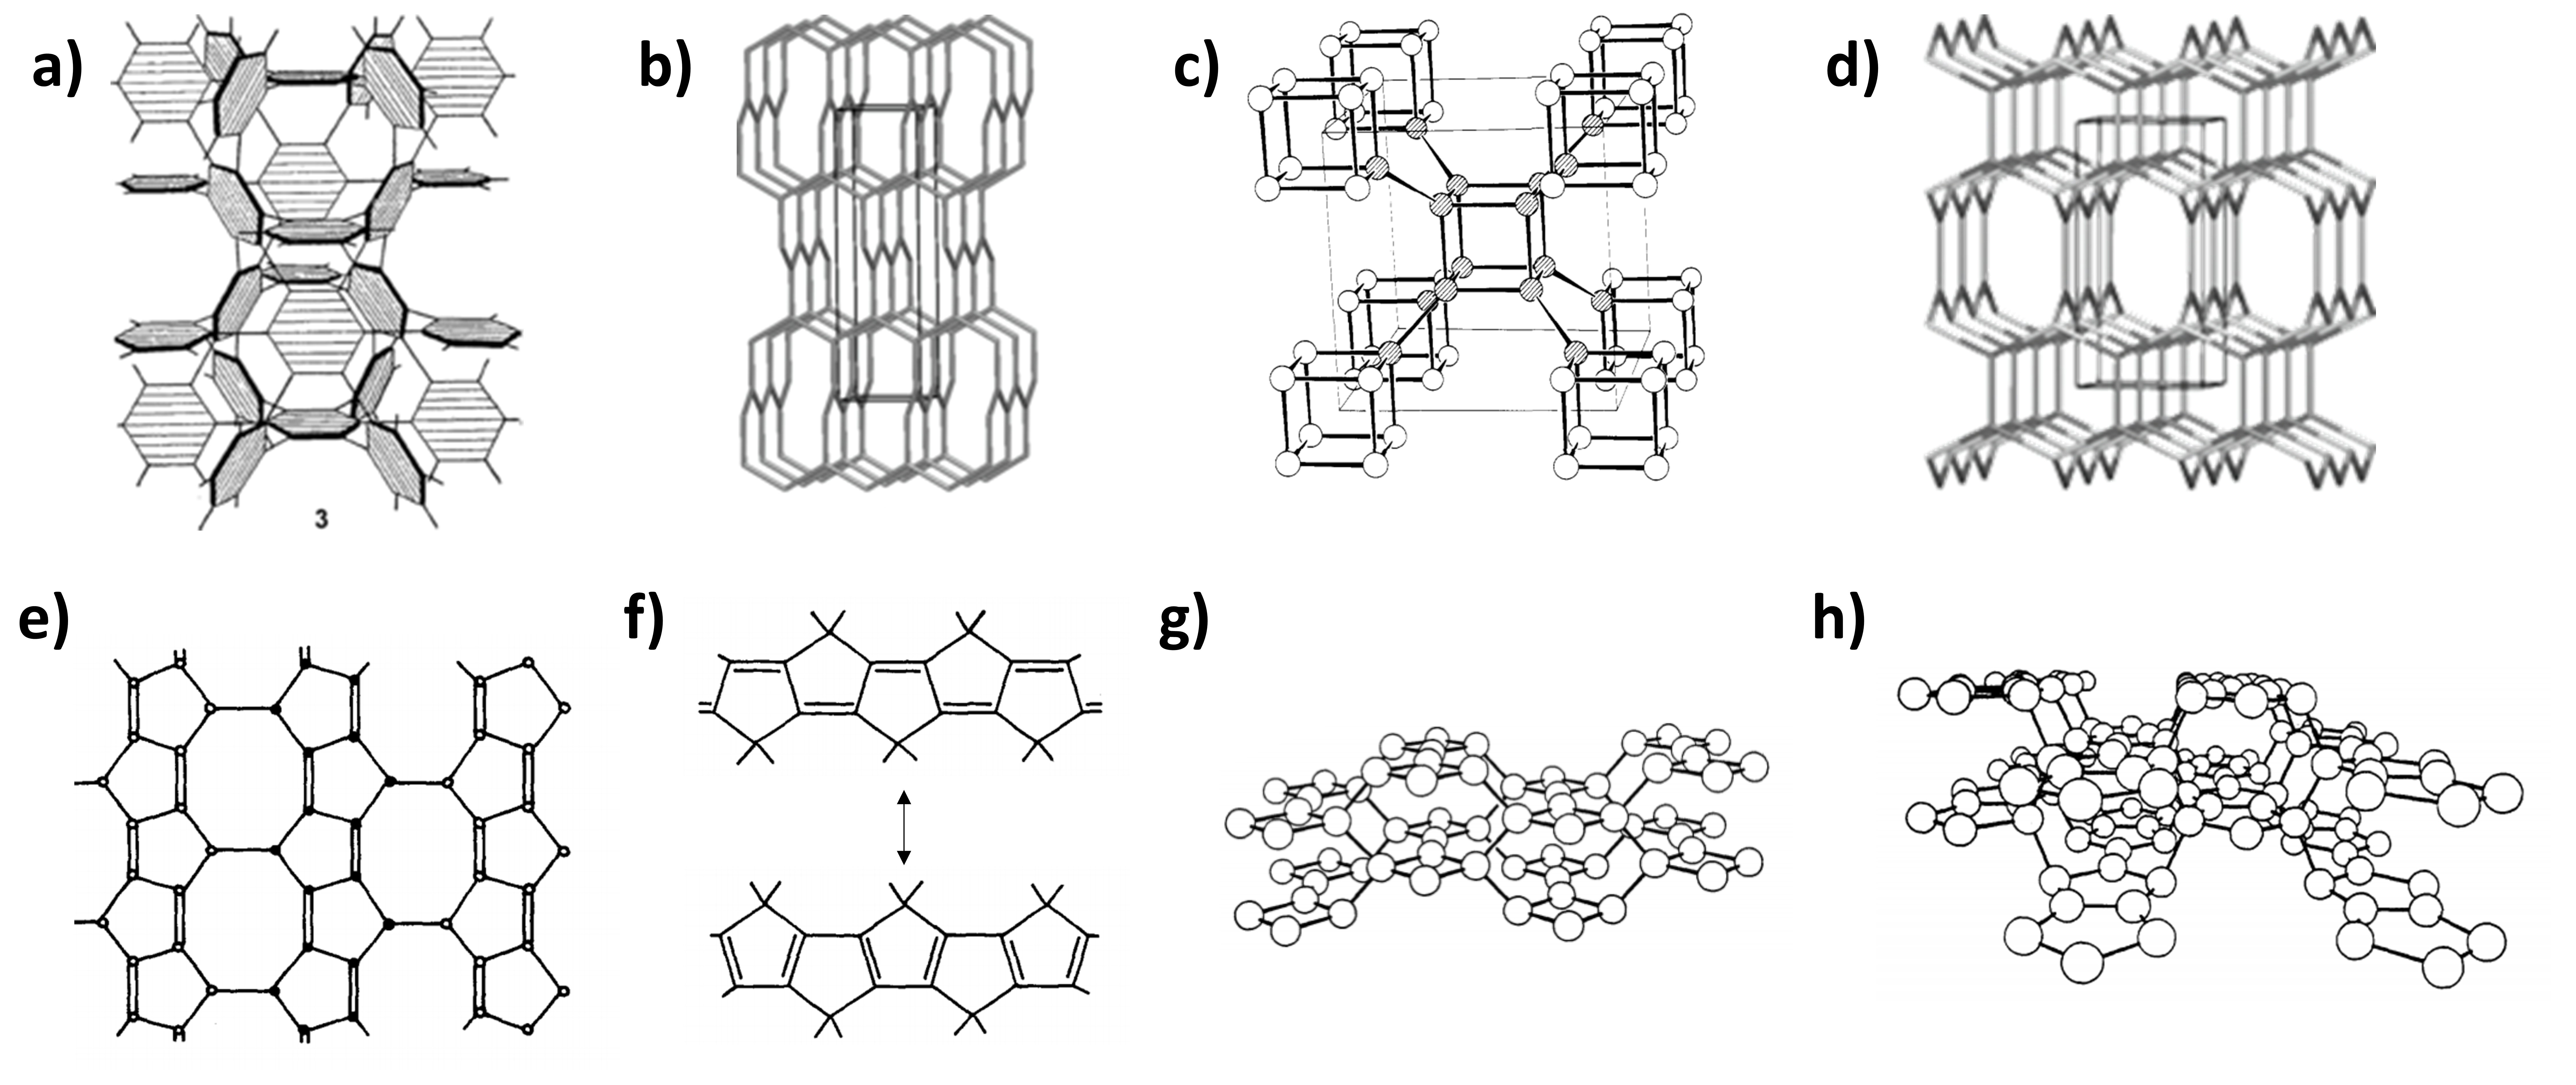
\includegraphics[width=1\linewidth]{capitulos/fig/intro/alotropos_hipoteticos}
			\caption{Representação de diversas estruturas alotrópicas hipotéticas propostas para o carbono.}
			\label{alotropos_hip}
		\end{figure}
	
		Com o advento e popularização dos cálculos de estrutura eletrônica a partir da década de 1980, diversas formas alotrópicas puramente hipotéticas puderam ter sua estrutura e suas propriedades exploradas. Um dos primeiros trabalhos desse tipo foi publicado por \citeauthor{hoffmann1983hypothetical} em \citeyear{hoffmann1983hypothetical}\footnote{Em seu artigo original Hoffmann não apresenta detalhes da metodologia computacional utilizada}, onde foi apresentada uma nova estrutura - chamada posteriormente de \textbf{bct-4} - composta somente por átomos de carbono $sp^2$ formando um novo alótropo de carbono metálico, com uma célula unitária tetragonal com grupo espacial \textit{I4\textsubscript{1}/amd} e grupo pontual $D^{19}_{4h}$ em uma rede 3-c $10^3$-\textbf{ths}\footnote{Seguindo a notação de redes periódicas proposta por \citeauthor{o2008reticular}} (\autoref{alotropos_hip}-\textbf{b}). Em \citeyear{johnston1989superdense} uma outra forma alotrópica, denominada \textbf{C\textsubscript{8}} foi proposta sendo formada por átomos de carbono formando cubos conectados pelo vértice (\autoref{alotropos_hip}-\textbf{c}), gerando um alótropo de carbono com alta densidade (0.338 mol/cm$^3$ contra 0.295 mol/cm$^3$ para o diamante). Em \citeyear{bucknum1994hypothetical} mais uma estrutura foi proposta por \citeauthor{bucknum1994hypothetical}, sendo formada por unidades 1,4-ciclohexadienoides em uma rede 3,4-c \textbf{tfi}, denominada spirographite (\autoref{alotropos_hip}-\textbf{d}). 
	
		Em \citeyear{balaban1989carbon} \citeauthor{balaban1989carbon} publicou um extenso trabalho explorando aspectos estruturais e da simetria de diversas estruturas alotrópicas de carbono. Nesse trabalho ele analisou as possíveis propriedades eletrônicas e propôs maneiras de nomear as diversas estruturas resultantes baseando-se na teoria de grafos, resultando em um belo sinergismo entre química e matemática. Esse trabalho pioneiro mostrou matematicamente que, devido às diferentes hibridações possíveis do átomo de carbono, o número de estruturas alotrópicas geradas pela combinação dessas diferentes formas é extremamente grande. Algumas das estruturas propostas por \citeauthor{balaban1989carbon} estão representadas na \autoref{alotropos_hip}-\textbf{e-h}.
		
		Diederich em \citeyear{diederich1992synthetic} \cite{diederich1992synthetic} e \citeyear{diederich1994carbon} \cite{diederich1994carbon, diederich1994synthetic} fez importantes contribuições à classe de novos alótropos de carbono. Através de uma meticulosa revisão da literatura e propostas criativas de novas estruturas, Diederich ajudou a construir uma biblioteca de reações que podem ser capazes de trazer diversas estruturas hipotéticas à realidade. De fato esse trabalho foi especialmente importante na preparação e observação do cyclo[18]carbon\cite{kaiser2019sp}, o mais recente alótropo de carbono relatado na literatura, demonstrando que a predição teórica da novas estruturas pode levar a sua futura obtenção experimental.
		
		Os trabalhos de Hoffmann, Balaban e Diederich abriram caminho e serviram como base e inspiração para que diversos pesquisadores investissem na busca computacional de novas estruturas alotrópicas, o foco principal do presente trabalho.
	
	\section{Alótropos com alta dureza}
	
		O diamante é conhecido principalmente por sua elevada dureza, sendo o material natural mais duro conhecido. Essa propriedade é resultado do tipo e natureza das ligações entre os átomos deste sólido. As ligações do tipo covalente são, em geral, muito mais fortes do que as apresentadas nos sólidos iônicos, e a geometria das ligações faz com que qualquer força em um átomo seja distribuída espacialmente para outros três átomos de maneira simétrica. Sua dureza medida na escala de Vickers é de 96$\pm$5 GPa e seu módulo Bulk é 443 GPa \cite{andrievski2001superhard}.  Inspirado no diamante, muitas pesquisas têm sido feitas na busca por novas estruturas de carbono com dureza próxima ou maior. 
				
		\begin{figure}[!h]
			\centering
			\includegraphics[width=.7\linewidth]{capitulos/fig/intro/superhard}
			\caption{Representação esquemática das estruturas de (a) bct-C$_4$, (b) M-Carbon, (c) T-Carbon, (d) W-Carbon e (e) Cco-C$_8$}
			\label{superhard}
		\end{figure}
	
		Em \citeyear{li2009superhard} \citeauthor{li2009superhard} identificaram a estrutura hipotética de um alótropo monoclínico com grupo espacial $C2/m$ utilizando busca evolucionária estrutural \cite{oganov2006crystal}. Essa estrutura, denominada M-Carbon, \autoref{superhard}-\textbf{b}, apresenta módulo Bulk calculado de 431.2 GPa e dureza calculada de 83.1 GPa, valores próximos do apresentado pelo diamante. 
		
		Em \citeyear{umemoto2010body} \citeauthor{umemoto2010body} identificaram mais uma fase cristalina composta somente por átomos de carbono com hibridação $sp^3$ a partir de simulações de dinâmica molecular da compressão de nanotubos de carbono do tipo (2,2). A estrutura resultante, denominada bct C$_4$, \autoref{superhard}-\textbf{a}, apresenta uma célula unitária tetragonal de corpo centrado com grupo pontual $I_4/mmm$ e módulo Bulk calculado de 428.7 GPa.
		
		Em \citeyear{wang2011low} \citeauthor{wang2011low} propuseram a estrutura de um alótropo ortorrômbico de corpo centrado com grupo espacial $Pmna$ e grupo pontual $D^{16}_{2h}$. Essa estrutura denominada W-Carbon, \autoref{superhard}-\textbf{d}, apresenta módulo Bulk de 444.5 GPa. No mesmo ano \citeauthor{zhao2011novel} propuseram a estrutura de um alótropo ortorrômbico de corpo centrado com grupo espacial $Cmmm$. Essa estrutura, denominada Cco-C\textsubscript{8} (\autoref{superhard}-\textbf{e}) é composta somente por átomos de carbono $sp^3$ e apresenta dureza calculada de 95.1 e módulo Bulk de 441 GPa. 
		
		Ainda em \citeyear{sheng2011t} \citeauthor{sheng2011t} propuseram a formação de um novo alótropo de carbono substituindo cada átomo de carbono da estrutura do diamante por uma unidade derivada de um tetraedrano, molécula hipotética em que cada vértice de um tetraedro é um átomo de carbono, formando o T-Carbon (\autoref{superhard}-\textbf{c}). A estrutura resultante se apresenta em uma célula unitária cúbica de corpo centrado com grupo pontual Fd$\bar{3}$m, possuindo módulo Bulk calculado de 169 GPa e dureza de 61.1 GPa. Esse alótropo foi obtido experimentalmente em \citeyear{zhang2017pseudo} por \citeauthor{zhang2017pseudo} através da conversão de nanotubos de carbono irradiados por laser e por \citeauthor{xu2020preparation} em \citeyear{xu2020preparation} através de deposição química de vapor (CVD). Esse é mais um ótimo exemplo de como a busca computacional de novos alótropos pode incentivar e guiar sua obtenção experimental.
		
		Em \citeyear{tian2012superhard} \citeauthor{tian2012superhard} utilizaram uma metodologia de otimização do tipo "\textit{particle-swarm}" para obter a estrutura hipotética de um alótropo monoclínico com simetria P2/m (C$^{1}_{2h}$). Essa estrutura, denominada F-Carbon (\autoref{superhard}-\textbf{f}) é composta somente por átomos de carbono sp$^3$ e apresenta dureza calculada de 93.9 GPa e módulo Bulk de 410 GPa.
		
		Com o avanço do tempo e a crescente atenção dada a essas estruturas, muitos grupos começaram a investir em generalizar conceitos e criar famílias de novos alótropos. \citeauthor{niu2012families} propuseram uma família composta por P-, R- e S-Carbon. 
	
	\section{Alótropos com propriedades eletrônicas especiais}
	
		Em \citeyear{baughman1987structure} \citeauthor{baughman1987structure} propuseram a existência de um conjunto de alótropos de carbono lamelares, sendo formados por átomos com hibridações $sp^2$ e $sp$. Esse é um dos primeiros exemplos de aplicação de uma regra estrutural sistemática na construção de estruturas estendidas. A estratégia principal é de substituir as ligações entre os anéis benzênicos ou entre as ligações duplas do grafite por unidades acetilênicas (-C$\equiv$C-), gerando três estruturas denominadas $\alpha$, $\beta$ e $\gamma$ grafino\footnote{Traduzindo livremente do original em inglês \textit{graphyne}}. Algumas dessas estruturas já haviam sido preditas em \citeyear{balaban1968chemical} por \citeauthor{balaban1968chemical}, porém não foram exploradas profundamente. O conceito do grafino pode ser generalizado considerando a substituição das ligações entre os anéis benzênicos do grafite por $n$ unidades acetilênicas, gerando assim a família dos $n$-grafinos. O 2-grafino, também chamado de grafidiino, foi sintetizado em \citeyear{li2010architecture} por \citeauthor{li2010architecture}.
		
		\citeauthor{baughman1987structure} consideraram em seus cálculos uma estrutura tridimensional lamelar, como a do grafite. Apesar de essa ser a forma mais estável para esses alótropos, após a observação experimental do grafeno uma corrida foi iniciada pela descoberta de novas estruturas bidimensionais com propriedades extraordinárias. \citeauthor{kim2012graphyne} mostraram através de cálculos DFT e \textit{tight-binding} que  $\alpha$- e $\beta$-1-grafino (\autoref{graphyne}-b e c) apresentam cones de Dirac em seu diagrama de bandas, com velocidades de Fermi dos elétrons próximas ao apresentado pelo grafeno. O $\gamma$-1-grafino (\autoref{graphyne}-d) apresenta um \textit{band gap} pequeno, de aproximadamente 0.47 eV, que diminui com o aumento do comprimento da ligação tripla e chega à zero quando o comprimento é de 1.278 Å.
		
		\begin{figure}[!h]
			\centering
			
\includegraphics[width=1\linewidth]{capitulos/fig/intro/graphyne}
			\caption{Representação esquemática e diagrama de bandas de (a) Grafeno, (b) $\alpha$-1-grafino, (c) $\beta$-1-grafino e (d) $\gamma$-1-grafino, (e) 6,6,12-grafino.}
			\label{graphyne}
		\end{figure}
	
		Uma quarta variante dessa estrutura explorada por \citeauthor{malko2012competition} em \citeyear{malko2012competition}, o 6,6,12-grafino (\autoref{graphyne}-e), apresenta dois cones de Dirac \footnote{Quando materiais apresentam bandas de valência e de condução se cruzando de maneira que lembra um cone em energias próximas do nível de Fermi ele pode apresentar propriedades eletrônicas especiais. Esse cruzamento recebe o nome de cone de Dirac.} em seu diagrama de bandas, um primeiro levemente abaixo do nível de Fermi e um segundo logo acima do nível de Fermi.\cite{malko2012competition} Esse fenômeno é resultado de uma auto-dopagem, no sentido de que no primeiro cone os elétrons se apresentam como portadores de carga e no segundo os buracos se apresentam como portadores de carga. Além disso, os cones apresentam formatos diferentes, indicando que as propriedades eletrônicas devido à esse fenômeno podem apresentar dependência direcional. 
		
		Outra curiosidade interessante é que a incidência de cones de Dirac está fortemente relacionada com estruturas que apresentam simetria hexagonal (p6m)\cite{wehling2014dirac}, entretanto essa estrutura apresenta dois cones de Dirac mesmo possuindo simetria retangular (pmm).
		
		A busca por propriedades eletrônicas excepcionais se estendeu além da procura por férmions topológicos de Dirac em sistemas 2D, tendo recentemente crescido na direção de fases topológicas exóticas como isolantes topológicos (materiais em que o \textit{Bulk} é isolante mas as bordas são condutoras), \textit{"nodal loop semimetals"} (sistemas 3D onde as bandas de valência e condução se tocam em \textit{loops} fechados e espaço dos momentos), ou \textit{"nodal point semimetals"} (materiais onde a superfície de Fermi possui dimensão zero e é conectada por arcos de Fermi na superfície da zona de Brillouin).  
		
		%\begin{figure}[!h]
			%\centering
			%
\includegraphics[width=1\linewidth]{capitulos/fig/intro/topologicos_3D}
			%\caption{Representação esquemática e diagrama de bandas de (a) %Pentagon-Carbon, (b) $\alpha$-1-grafino, (c) $\beta$-1-grafino e (d) %$\gamma$-1-grafino, (e) 6,6,12-grafino.}
		%	\label{topologicos_3d}
		%\end{figure}
		
		Em \citeyear{zhong2017three} \citeauthor{zhong2017three}  apresentaram uma fase metaestável tridimensional composta por anéis pentagonais de carbono conectados perpendicularmente. Essa estrutura, que apresenta grupo espacial \textit{I4\textsubscript{1}/amd} e grupo pontual $D^{19}_{4h}$, já havia sido imaginada por \citeauthor{balaban1989carbon}, porém não havia até então tido sua estrutura eletrônica explorada de maneira mais profunda. Em seu trabalho, os autores mostraram que esse material apresenta férmions topológicos emergentes, no qual quando aplicando-se uma deformação na estrutura o Pentagon Carbon apresenta uma transição de fase topológica passando de férmions tripleto isospin-1 para férmions triplamente degenerados e para férmions do tipo Hopf-link Weyl-loop.
	
	\section{Outras estruturas 3D}
	
		O conceito de inserir unidades do tipo -C$\equiv$C-, utilizando para a idealização dos $n$-grafinos, foi explorado também de maneira independente por \citeauthor{jo2012carbon} em \citeyear{jo2012carbon} para propor a estrutura do Y-Carbon e híbridos entre o Y-Carbon e o T-Carbon, através da inserção de uma unidade de acetileno entre cada átomo de carbono da estrutura do diamante, e por \citeauthor{balaban2013expanded} em \citeyear{balaban2013expanded} para criar uma miríade de estruturas hipotéticas, combinando diversos motivos estruturais. Em \citeyear{costa2018n} nosso grupo também fez uma importante contribuição, generalizando o conceito da inserção de $n$ unidades de acetileno entre os átomos $sp^3$ do diamante e criando a família dos $n$-diamantinos\cite{costa2018n}, sendo o Y-Carbon um membro dessa família denominado 1-diamantino. 
	

	
	
	




% ----------------------------------------------------------
% Capítulos
% ----------------------------------------------------------


%% abtex2-modelo-include-comandos.tex, v-1.9.6 laurocesar
%% Copyright 2012-2016 by abnTeX2 group at http://www.abntex.net.br/ 
%%
%% This work may be distributed and/or modified under the
%% conditions of the LaTeX Project Public License, either version 1.3
%% of this license or (at your option) any later version.
%% The latest version of this license is in
%%   http://www.latex-project.org/lppl.txt
%% and version 1.3 or later is part of all distributions of LaTeX
%% version 2005/12/01 or later.
%%
%% This work has the LPPL maintenance status `maintained'.
%% 
%% The Current Maintainer of this work is the abnTeX2 team, led
%% by Lauro César Araujo. Further information are available on 
%% http://www.abntex.net.br/
%%
%% This work consists of the files abntex2-modelo-include-comandos.tex
%% and abntex2-modelo-img-marca.pdf
%%

% ---
% Este capítulo, utilizado por diferentes exemplos do abnTeX2, ilustra o uso de
% comandos do abnTeX2 e de LaTeX.
% ---

\chapter{Objetivos}

O principal objetivo deste trabalho é explorar a utilização de métodos de cálculos baseados na Teoria do Funcional da Densidade (DFT) para diferentes estruturas alotrópicas do carbono, prevendo a existência de novas estruturas e suas possíveis propriedades estruturais, eletrônicas e vibracionais. 

Esse trabalho pode ser resumido em três principais perguntas:

\begin{enumerate}
	
	\item[1$^{\circ}$:] É possível utilizar métodos DFT para predizer a estrutura e propriedades de diferentes alótropos de carbono?
		\subitem $\bullet$ Qual o melhor funcional DFT?
		\subitem $\bullet$ Correções de energia de dispersão são necessária?
	
	\item[2$^{\circ}$:] É possível propor novas estruturas alotrópicas metaestáveis para o carbono baseadas em motivos estruturais moleculares?
		\subitem $\bullet$ É possível propor alótropos de carbono com base na estrutura do spiropentadieno?
		\subitem $\bullet$ É possível propor alótropos combinando motivos estruturais, como o motivo spiro, e átomos de carbono com uma hibridização específica?

	\item[3$^{\circ}$:] É possível utilizar formas alotrópicas já existentes, como por exemplo o carbino, como “blocos de construção” para novos alótropos de carbono?
	
\end{enumerate}


\part{Metodologia}

\include{capitulos/3-metodologia}

\part{Resultados \& Discussão}

\include{capitulos/4-resultados}

%% abtex2-modelo-include-comandos.tex, v-1.9.6 laurocesar
%% Copyright 2012-2016 by abnTeX2 group at http://www.abntex.net.br/ 
%%
%% This work may be distributed and/or modified under the
%% conditions of the LaTeX Project Public License, either version 1.3
%% of this license or (at your option) any later version.
%% The latest version of this license is in
%%   http://www.latex-project.org/lppl.txt
%% and version 1.3 or later is part of all distributions of LaTeX
%% version 2005/12/01 or later.
%%
%% This work has the LPPL maintenance status `maintained'.
%% 
%% The Current Maintainer of this work is the abnTeX2 team, led
%% by Lauro César Araujo. Further information are available on 
%% http://www.abntex.net.br/
%%
%% This work consists of the files abntex2-modelo-include-comandos.tex
%% and abntex2-modelo-img-marca.pdf
%%

% ---
% Este capítulo, utilizado por diferentes exemplos do abnTeX2, ilustra o uso de
% comandos do abnTeX2 e de LaTeX.
% ---

\chapter{Novos Alótropos de Carbono}
\label{chap:novos_alotropos}
\section{Spiro-Carbon}
\label{sec:spiro}

	Em um trabalho desenvolvido pelo nosso grupo anteriormente ao desenvolvimento desta dissertação, foi explorada a existência de uma nova família de alótropos de carbono, denominada \textit{n}-diamantinos, sendo relatada em artigo publicado em \citeyear{costa2018n} \cite{costa2018n}. Esta família descreve uma generalização do conceito de formação de novas estruturas de carbono através da inserção de \textit{n} derivados de acetileno entre os átomos de carbono. 
	
	Se considerarmos que um dos membros desta família, o 1-diamantino que também relatado na literatura como Y-Carbon \cite{jo2012carbon}, poderia sofrer um rearranjo entre as ligações triplas vicinais (com mostrado na \autoref{soliton}),o  resultado seria a formação de dois anéis de três membros perpendiculares compartilhando um átomo de carbono entre si, um motivo estrutural conhecido como \textit{spiro}. Esse motivo estrutural resultante estaria conectado por ligações químicas formando uma estrutura periódica.

	\begin{figure}[ht]
		\centering
		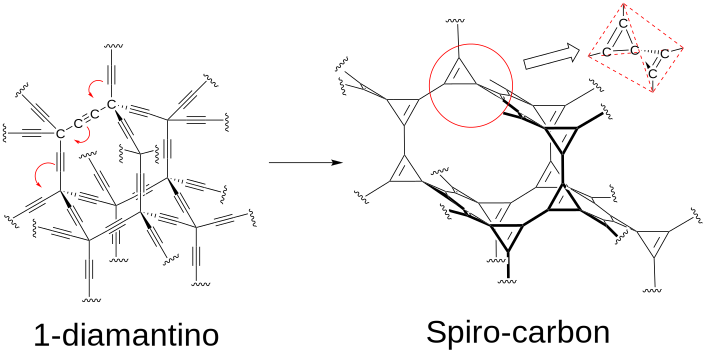
\includegraphics[width=1\linewidth]{capitulos/fig/results1/estrutura_1diamantino-spiro.eps}
		\caption{Rearranjo das cadeias geminais do 1-diamantino para formar um novo alótropo de carbono com o motivo estrutural \textit{spiro}.}
		\label{soliton}
	\end{figure}

	A síntese composto molecular que apresenta o motivo estrutural que forma esta estrutura, o spiropentadieno, já foi relatada na literatura em \citeyear{billups1991spiropentadiene} por \citeauthor{billups1991spiropentadiene}.\footnote{A estrutura desta molécula é apresentada em mais detalhes no Apêndice \autoref{chap:spiropentadiene}} Além disso, algumas variações estruturais dessa molécula já apresentaram propriedades interessantes. Ela já foi explorada, por exemplo, para propor um hidrocarboneto que poderia violar o paradigma químico de mais de 150 anos de que um átomo de carbono tetravalente e tetra-coordenado deve assumir um arranjo estrutural tetraédrico \cite{esteves2005neutral}. 
	
	No spiropentadieno neutro, dois anéis de três membros estão ortogonais entre sí, o que faz dessa molécula uma espécie tetraedro esticado. Dessa forma, poderíamos ligar esses tetraedros de uma maneira análoga à ligação dos átomos de carbono no diamante, gerando assim a estrutura de um novo alótropo de carbono.

	\subsection{Estrutura}

	A estrutura desse novo alótropo de carbono, denominada de Spiro-Carbon, contém 10 átomos em uma célula unitária primitiva tetragonal de corpo centrado, apresentando grupo espacial $I4_1/amd$ (\#141) e grupo pontual $D_{4h}$. A geometria resultante da otimização estrutural apresenta os parâmetros de célula \textit{a} = \textit{b} = 5.122 \AA{}, \textit{c} = 13.126 \AA{} e $\alpha$ = $\beta$ = $\gamma$ = 90$^\circ$, apresentando densidade de 1.16 g/cm$^3$. Representações da célula unitária vista por pelos diferentes vetores de célula são mostradas na \autoref{estrutura_spiro}
	
	\begin{figure}[hbt!]
		\centering
		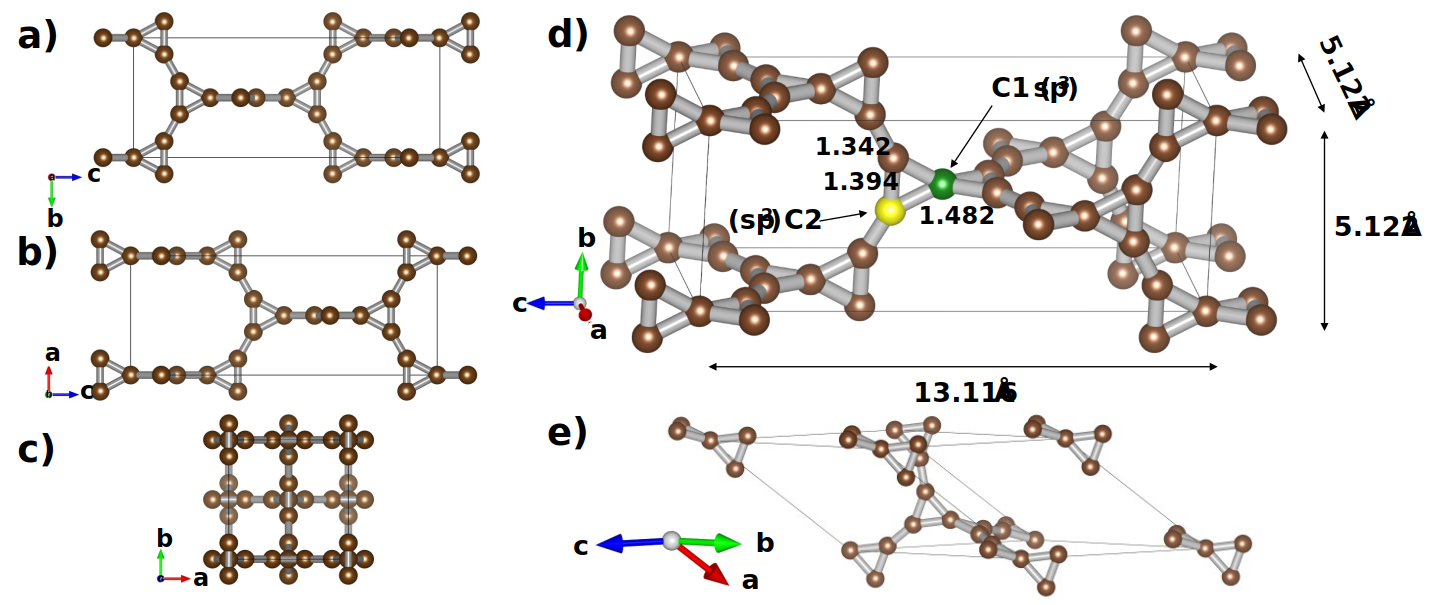
\includegraphics[width=1\linewidth]{capitulos/fig/results1/estrutura_spiro}
		\caption{Representação atômica da estrutura tetragonal do Spiro-Carbon ao longo dos eixos $a$, $b$ e $c$ (\textbf{a)} - \textbf{c)}). \textbf{d)} Representação atômica da estrutura tetragonal do Spiro-Carbon. Por simplicidade é mostrado a célula tetragonal simples, contendo duas fórmulas unitárias por cela. Essa simplificação ajuda no entendimento da estrutura de forma mais intuitiva. \textbf{e)} célula primitiva tetragonal de corpo centrado.}
		\label{estrutura_spiro}
	\end{figure}

	Baseado nos elementos de simetria apresentados pelo Spiro-Carbon, os dois átomos não equivalentes ocupam as posições de Wyckoff \textit{4a} e \textit{16h}, estando \textbf{C1} (destacado em verde) no sítio \textit{4a} com coordenadas fracionárias (0, 0, 0) e \textbf{C2} (destacado em amarelo) no sítio \textit{16h}, com coordenadas fracionárias (0.00000,  0.13609,  0.09971). Analisando a estrutura otimizada é possível distinguir três diferentes tipos de ligação, como representado na \autoref{estrutura_spiro}-d): \textit{i)} As ligações conectando o carbono $sp^3$ central aos seus vizinhos (C1-C2), com comprimento de 1.482 \AA{}, similar às ligações equivalentes na estrutura de seu análogo molecular spiropentadieno\footnote{Os cálculos para a molécula spiropentadieno são apresentadas no \autoref{chap:spiropentadiene}} (que apresenta 1.483 \AA{}) e apresentando comprimento compatível com ligações C-C simples; \textit{ii)} as ligações entre os átomos de carbono $sp^2$ (C2-C2) com comprimento de ligação de 1.394 \AA{}, consideravelmente maior do que a ligação correspondente no spiropentadieno (1.31 \AA{}) e apresentando um caráter intermediário entre ligações simples e duplas, algo típico de ligações duplas conjugadas \cite{lide1962survey}; \textit{iii)} as ligações que conectam os motivos estruturais spiro para formar a estrutura polimérica (C2=C2), com comprimento de ligação de 1.342 \AA, característico de ligações duplas C=C \cite{zavitsas2003relation,lide1962survey}.  
	
	Os ângulos entre os anéis de três membros na porção \textit{spiro} são de 90$^\circ$, mesmo de seu análogo molecular. Os ângulos internos são 62$^\circ$ (C1-C2-C2 e C2-C2-C1) e 56$^\circ$ (C2-C1-C2), levemente diferentes dos apresentados pelo análogo molecular, 63.6$^\circ$ e 52.8$^\circ$ respectivamente. Essa pequena diferença pode ser explicada pelo aumento do comprimentos das ligações endo-anulares (C2-C2), decorrente da formação da estrutura periódica, de forma a aliviar a tensão anular. 
			
	Essa modificação nos comprimentos e ângulos de ligação na porção \textit{spiro}, que resulta da formação da ligação dupla exo-anular em vez da endo-anular como no composto molecular, contribui para uma redução da tensão de anel nesta porção da estrutura e promove um aumento da estabilidade estrutural da forma cristalina. Além disso, essa modificação no perfil das ligações químicas pode gerar consequências interessantes na estrutura eletrônica desse novo alótropo de carbono, como será explorado posteriormente.
	
	Uma forma interessante de visualizar a estrutura do Spiro-Carbon é imaginar esse alótropo como sendo um arranjo perpendicular de fios condutores de \textit{cis}-(poli)acetileno "unidos" por átomos de carbono $sp^3$, como apresentado na \autoref{spiro_fios}.
	
	\begin{figure}[ht]
		\centering
		\includegraphics[width=.7\linewidth]{capitulos/fig/results1/column5.png}
		\caption{Representação esquemática do Spiro-Carbon, destacando seu caráter análogo a fios condutores de \textit{cis}-(poli)acetileno "unidos" por átomos de carbono $sp^3$.}
		\label{spiro_fios}
	\end{figure}
	
	\subsection{Estabilidade Relativa e Propriedades Mecânicas}
	
	Para investigar a estabilidade relativa da nova estrutura proposta, foi calculada a dispersão de fônons ao longo de um caminho entre pontos de alta simetria na primeira zona de Brillouin \cite{bradley2010mathematical}. Como pode ser observado na \autoref{phDOS_EoS}-a), nenhuma frequência imaginária foi encontrada, confirmando que a estrutura do Spiro-Carbon corresponde a um mínimo na superfície de energia potencial. 
	
	\begin{figure}[ht]
		\centering
		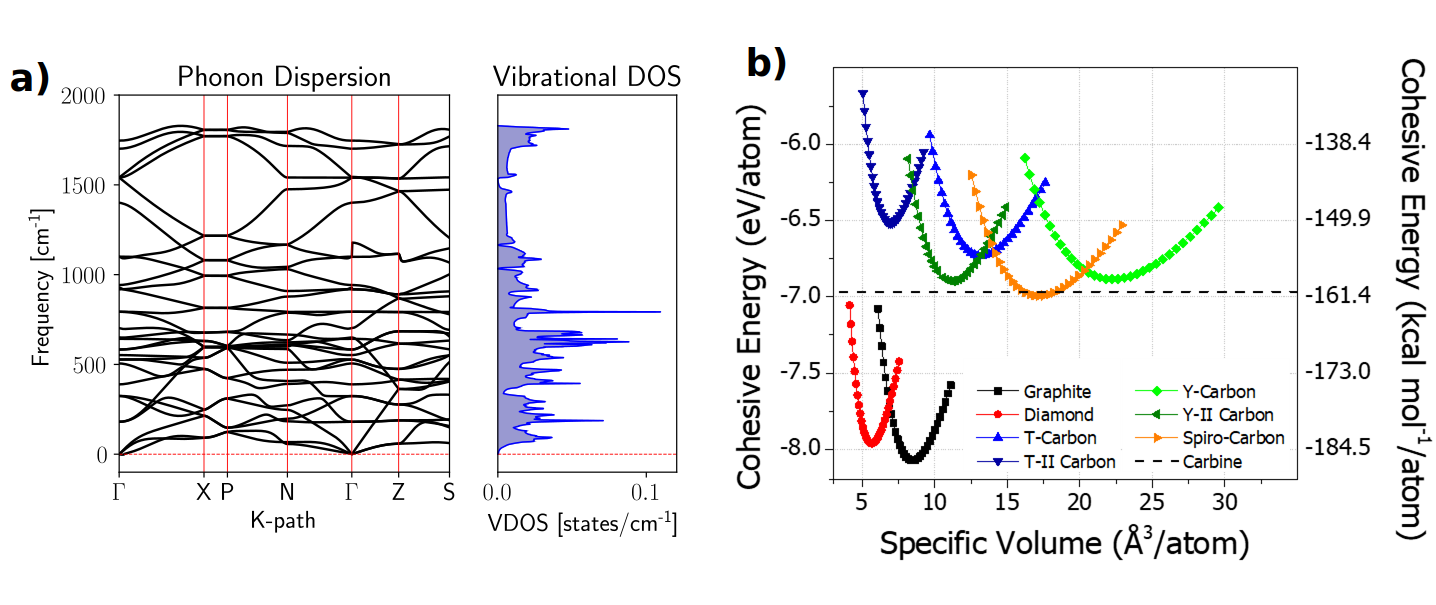
\includegraphics[width=1\linewidth]{capitulos/fig/phDOS_EoS}
		\caption{a) Gráfico da dispersão de fônons ao longo de alguns pontos de alta simetria na primeira zona de Brillouin e a correspondente densidade de estados vibracionais (VDOS). Inserto: Caminho através dos pontos de alta simetria da primeira zona de Brillouin. b) Energia coesiva por átomo em função do volume ($E_c(V)$) por átomo para diferentes alótropos de carbono. do Spiro-Carbon}
		\label{phDOS_EoS}
	\end{figure}

	Para aprofundar o entendimento sobre a estabilidade termodinâmica relativa do Spiro-Carbon, a \autoref{phDOS_EoS}-b) mostra a variação da energia coesiva em função do volume (ambos por átomo) para diferentes alótropos de carbono. Como esperado, a curva $E_c(V)$ para o Spiro-Carbon apresenta claramente um mínimo correspondente ao estado meta estável desta estrutura com menor energia coesiva do que o grafite e o diamante. Apesar disso, o Spiro-Carbon se mostrou mais estável do que outros alótropos de carbono 3D (exceto, é claro, diamante e grafite), como o 1-diamantino/Y-Carbon \cite{costa2018n,li2014modulated}, por aproximadamente 2.3 kcal/mol (0.1 eV) por átomo e o T-Carbon \cite{sheng2011t} por aproximadamente 6.1 kcal/mol (0.26 eV), como mostrado na \autoref{energy}. Esse fato é especialmente encorajador, considerando que recentemente a síntese do T-Carbon foi reportada por \citeauthor{zhang2017pseudo}, utilizando uma suspensão em metanol de nanotubos de carbono \textit{multi-wall} irradiados com laser pulsado em picosegundos.
	
	\begin{table*}[ht]
		\centering
		\renewcommand{\arraystretch}{1.1}
		\caption{Módulo das energias relativa e coesiva por átomo para o Spiro-Carbon comparado com diferentes alótropos de carbono.}
		\label{energy}
		\begin{tabular}{lcccc}
			\hline
			\hline
			\multicolumn{1}{c}{\multirow{2}{*}{Estrutura}} & \multicolumn{2}{c}{Energia Relativa} & \multicolumn{2}{c}{Energia Coesiva}                             \\ \cline{2-5} 
			\multicolumn{1}{c}{}                           & \multicolumn{1}{l}{eV/átomo} & \multicolumn{1}{l}{kcal/mol/átomo} & \multicolumn{1}{l}{eV/átomo} & \multicolumn{1}{l}{kcal/mol/átomo} \\ \hline
				Grafite      & 0.000  & 0.000  & 7.856  & 181.16  \\
				Diamante     & 0.112  & 2.57   & 7.744  & 178.59  \\
				Spiro-Carbon & 1.079  & 24.88  & 6.777  & 156.29  \\
				Carbino      & 1.106  & 25.50  & 6.750  & 155.67  \\
				Y Carbon     & 1.189  & 27.41  & 6.667  & 153.75  \\
				Y-II Carbon  & 1.177  & 27.15  & 6.679  & 154.01  \\
				T Carbon     & 1.342  & 30.94  & 6.514  & 150.22  \\
				T-II Carbon  & 1.554  & 35.84  & 6.302  & 145.32  \\ \hline \hline
		\end{tabular}
	\end{table*}
	
	
	Avaliando agora a estabilidade mecânica da nova estrutura proposta, as seis constantes elásticas ($\textbf{C}_{ij}$ em GPa) foram calculadas e são apresentadas na \autoref{elastic}.
	
	\begin{table}[ht]
		\centering
		\renewcommand{\arraystretch}{1.1}
		\caption{Constantes elásticas ($\textbf{C}_{ij}$ in GPa), módulo Bulk (\textbf{B}), shear (\textbf{G}) e Young (\textbf{E}) (em GPa) e razão de Poisson ($\nu$) calculados para o Diamante, T-Carbon, 1-diamantino (Y-Carbon) e Spiro-Carbon}
		\label{elastic}
		\begin{tabular}{lccccc}
			\hline \hline
			                             & Diamante Exp.\textsuperscript{\cite{grimsditch1975brillouin}}     &Diamante Calc. & T-Carbon & 1-diamantino & Spiro-Carbon \\\hline
			\textbf{C\textsubscript{11}} &  1076.4 $\pm$ 0.2 & 1106.43 & 210.98 & 101.68      & 277.76       \\
			\textbf{C\textsubscript{33}} &	1076.4 $\pm$ 0.2 & 1106.43 & 143.75 & 101.68      & 308.54       \\
			\textbf{C\textsubscript{44}} &  577.4 $\pm$ 1.4  & 591.34  & 66.14 & 13.52       & 75.04        \\
			\textbf{C\textsubscript{66}} &  577.4 $\pm$ 1.4  & 591.34  & 66.14 & 13.52       & 3.61         \\
			\textbf{C\textsubscript{12}} & 	125.2 $\pm$ 2.3  & 153.08  & 143.75 & 79.58       & 3.36         \\
			\textbf{C\textsubscript{13}} &	125.2 $\pm$ 2.3  & 153.08  & 143.75 & 79.58       & 68.88        \\
			\textbf{B}                   &	442.27$\pm$ 1.53 &  470.86 & 166.62 & 86.94       & 123.73       \\
			\textbf{G}                   &	524.68$\pm$ 0.70 &  542.45 & 50.40 & 12.47       & 47.79        \\
			\textbf{E}                   & 1127.98$\pm$ 1.55 & 1175.83 & 137.30 & 35.71       & 121.98       \\
			\textbf{$\nu$}               &  0.075$\pm$ 0.048 &  0.084  & 0.362 & 0.43        & 0.276        \\
			\hline \hline
		\end{tabular}
		\noindent
	\end{table}
	
	As quatro condições necessárias e suficientes que devem ser satisfeitas, baseadas nos critérios de estabilidade de Born \cite{born1940stability}, para garantir a estabilidade mecânica para uma rede tetragonal são:
	
	\begin{equation*}
	C_{11} > |C_{12}|, \quad 2C_{13} < C_{33} (C_{11} + C_{12}),
	\end{equation*}
	\begin{equation*}
	C_{44} > 0, \quad C_{66} > 0
	\end{equation*}
	
	É possível verificar que todas elas são completamente satisfeitas. Adicionalmente, é pode-se examinar outros critérios que devem ser satisfeitos \cite{mouhat2014necessary}: 
	
	\begin{enumerate}
	    \item[(1)] A matriz \textbf{C} é positiva definida \footnote{Em álgebra linear, uma matriz definida positiva é uma matriz que, em muitos aspectos, é análoga a um número real positivo. A noção é parecida com a de uma forma bilinear simétrica positiva-definida (ou uma forma sesquilinear no caso complexo). A definição adequada de definida positiva não tem ambiguidades no caso de matrizes Hermitianas, mas não há consenso na literatura a respeito de como ela deve ser estendida para matrizes não Hermitianas, se é que isso deve ser feito.} ;
	    \item[(2)] Todos os autovalores de \textbf{C} são positivos;
	    \item[(3)] Todos os menores principais de \textbf{C} \footnote{determinantes das \textit{k} submatrizes da esquerda superior,para 1 $\leq$ \textit{k} $\leq$ 6} são positivos  (critério de Sylvester); e
	    \item[(4)] Um conjunto arbitrário de menores de \textbf{C} são positivos. 
	\end{enumerate}

	Todos esses critérios são satisfeitos pelo Spiro-Carbon, dessa forma podemos concluir que essa nova estrutura proposta é mecanicamente estável. 
	
	Para caracterizar o comportamento mecânico no regime elástico desta nova estrutura, uma análise tensorial completa da matriz elástica foi conduzida. Os valores médios das principais propriedades mecânicas foram calculadas segundo três diferentes métodos de aproximação e são apresentadas na \autoref{average_elastic}.
	
	\begin{table*}[!ht]
		\centering
		\renewcommand{\arraystretch}{1.5}
		\caption{Valores médios das principais propriedades mecânicas do Spiro-Carbon.}
		\label{average_elastic}
		\begin{tabular}{@{}ccccc@{}}
			\hline
			\hline
			Aproximação & Módulo     & Módulo de   & Módulo      & Razão de \\ 
			            & Bulk (GPa) & Young (GPa) & Shear (GPa) & Poisson \\ \hline
			Voigt       & 127.37 & 196.25 & 78.93 & 0.24 \\
			Reuss       & 124.06 &  44.86 & 15.58 & 0.44 \\
			Hill        & 125.71 & 125.98 & 47.25 & 0.33 \\\hline
			\hline
		\end{tabular}
	\end{table*}

	
	\begin{figure*}[!ht]
		\centering
		\includegraphics[width=1\linewidth]{capitulos/fig/elastic_2}
		\caption{Dependência espacial do (a) módulo de Young; (b) compressibilidade linear; (c) módulo Shear e (d) razão de Poisson.}
		\label{elastic_m}
	\end{figure*}
	
	A \autoref{elastic_m} mostra os gráficos da dependência espacial nos planos \textbf{xy}, \textbf{xz} e \textbf{yz} para os módulos de Young (\textbf{E}) e shear  (\textbf{G}), compressibilidade linear  ($\beta$) e razão de Poisson ($\nu$). A principal característica que podemos destacar é a grande anisotropia no plano \textbf{xy} para todas as propriedades, exceto a compressibilidade linear. Essa característica é comum para materiais porosos \cite{ortiz2012anisotropic} e pode ser um grande indicativo de que o Spiro-Carbon, quando sintetizado, se apresentará como um material altamente dúctil. 
	
	A anisotropia do módulo de Young, caracterizada pela razão A\textsubscript{E} = E\textsubscript{max}/E\textsubscript{min} é de 19.58. Os valores máximos dessa propriedade coincidem com as direções dos eixos \textit{x}, \textit{y} e \textit{z}, exibindo valor máximo de 274.78 GPa nessas direções. Em todas as outras direções do plano \textit{xy} os valores apresentados são excepcionalmente baixos, possuindo valore mínimo de 14.03 GPa. O módulo de cisalhamento, também conhecido como módulo de rigidez ou módulo de torção, também apresenta a mesma tendência, possuindo alta anisotropia, A\textsubscript{G} = 29.98, mas com seus valores máximos nas direções diagonais aos planos \textit{xy}, \textit{xz} e \textit{yz}. Os valores médios de todas as propriedades calculadas são apresentadas na \autoref{average_elastic}.
	
	Uma boa maneira de avaliar a dureza que o material policristalino poderia ter é utilizando o modelo empírico de \citeauthor{chen2011modeling}. Utilizando esse modelo, a dureza de Vicker obtida para o Spiro-Carbon é de 4,37 GPa (446 HV)\footnote{1 HV = 0.009807 GPa} valor muito mais baixo do que o para o diamante (90,9 GPa, 9266 HV) porém acima do apresentado pelo T-Carbon (1,89 GPa, 193 HV). Esse baixo valor de dureza indica que, uma vez sintetizado, esse material irá pertencer à classe de materiais maleáveis, uma característica interessante considerando a demanda crescente pelo desenvolvimento de materiais condutores e maleáveis \cite{kim2008stretchable, valentine2017hybrid, gong2017one}.
	%
	
	\subsection{Propriedades Eletrônicas}
	
	Como mencionado anteriormente, a estrutura do Spiro-Carbon se assemelha a um conjunto cadeias de \textit{trans-cisoide}-(poli)acetileno nos eixos \textit{x} e \textit{y} interconectados por átomos de carbono com hibridação $sp^3$. Uma vez que a cadeia de \textit{trans-cisoide}-(poli)acetileno isolada é um semi-condutor com \textit{band gap} de aproximadamente 1.3 eV \cite{baughman1982structural}, seria razoável imaginar que a estrutura eletrônica do Spiro-Carbon herdasse essa característica. Curiosamente ao analisar o diagrama de bandas, apresentado na \autoref{band1}, é possível observar que o Spiro-Carbon apresenta um caráter eletrônico metálico, devido à interseção entre as bandas de condução e de valência abaixo do nível de Fermi próximo ao ponto Z da zona de Brillouin. 
	
	
	\begin{figure}[!ht]
		\centering
			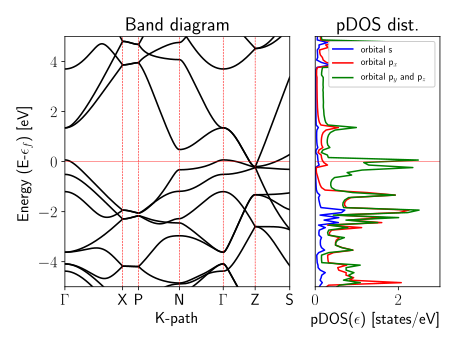
\includegraphics[width=.8\linewidth]{capitulos/fig/results1/bands_smearing}
		\caption{Dispersão de energia das bandas ao longo dos principais pontos de alta simetria na primeira zona de Brillouin (esquerda) e densidade de estados projetada nos orbitais (direita) para o Spiro-Carbon. A energia de Fermi ($\epsilon_f$) foi ajustada para 0.}
		\label{band1}
	\end{figure}

	A \autoref{pdos_byatom} apresenta a densidade de estados projetada (pDOS) referente a cada átomo que compõe a célula primitiva. É possível observar que o átomo \textbf{C2}, com hibridação $sp^2$ é o único que apresenta contribuição para a densidade de estados próxima do nível de Fermi. Isso pode ser um forte indicativo de que as ligações duplas conjugadas formadas por esses átomos sejam as principais responsáveis pelo caráter metálico deste material. 
	
	
	\begin{figure}[!ht]
		\centering
		\includegraphics[width=1.\linewidth]{capitulos/fig/results1/pdos_byatom0}
		\caption{Densidade de estados projetada para cada átomo da célula primitiva. Em cima para o átomo \textbf{C1} e em baixo para o átomo \textbf{C2}. A energia de Fermi ($\epsilon_f$) foi ajustada para 0.}
		\label{pdos_byatom}
	\end{figure}


	É apresentado na literatura que a cadeia de \textit{trans-}(poli)acetileno seria condutora se todas as ligações entre os átomos de carbono tivessem o mesmo comprimento, de 1,391 \AA{}, gerando assim uma cadeia infinita de ligações $\pi$ conjugadas. \cite{suhai1983bond, whangbo1979conjugated} De fato, cálculos feitos no mesmo nível dos apresentados até aqui confirmaram isso (Apêndice \ref{chap:bands_poliacetileno} - \autoref{bands_trans}). O caráter semi-condutor das cadeias de \textit{trans}-(poli)acetileno surgem do fato de que, em uma cadeia unidimensional infinita, o estado fundamental duplamente degenerado é instável devido à \textit{instabilidade de Peierls}\cite{peierls1996quantum}. Isso faz com que as ligações entre os átomos de carbono alternem entre simples e duplas, quebrando essa degenerescência e forçando os átomos de carbono a se agruparem em pares. Esse fenômeno, conhecido como \textbf{distorção de Peierls}, quebra a simetria translacional e separa os níveis de energia das bandas de valência e condução, convertendo a estrutura em um semi-condutor. \cite{peierls1996quantum}
	
	O \textit{cis}-(poli)acetileno apresenta o mesmo fenômeno, entretanto a distorção das ligações pode gerar duas formas: \textit{cis-transoide}-(poli)acetileno e \textit{trans-cisoide}-(poli)acetileno. Essas duas formas apresentam características eletrônicas parecidas, porém com \textit{band gap} diferentes. As formas \textit{cis}-(poli)acetileno e \textit{cis-transoide}-(poli)acetileno apresentam \textit{band gaps} de 0,8 eV, calculados com funcional PBE, enquanto a forma \textit{trans-cisoide}-(poli)acetileno apresenta band gap de 0,3 eV (para mais detalhes ver \autoref{chap:bands_poliacetileno}).
	
	Na estrutura do Spiro-Carbon as ligações conectando os átomos C2 apresentam comprimento de ligação de 1.342 \AA{} e 1.394 \AA{}, muito próximo dos apresentados pelo \textit{trans-cisoid}-(poli)acetileno, no qual as ligações correspondentes apresentam comprimentos de 1.377 \AA{} e 1.424 \AA{}. Esses valores estão de acordo com observações experimentais e cálculos teóricos reportados na literatura \cite{chien1982estimate, chien2012polyacetylene, whangbo1979conjugated}.
	
	\begin{figure}[!ht]
		\centering
		\includegraphics[width=.9\linewidth]{capitulos/fig/results1/poliacetileno_2_spiro}
		\caption{Diagrama de bandas das estruturas intermediárias entre o \textit{cis}-(poli)acetileno e o Spiro-Carbon}
		\label{acetileto_2_spiro}
	\end{figure}

	A \autoref{acetileto_2_spiro} apresenta o diagrama de bandas das estruturas intermediárias entre o \textit{cis}-(poli)acetileno e o Spiro-Carbon. É possível observar que conforme a cadeia lateral aumenta e se aproxima da forma estrutural do Spiro-Carbon, os orbitais $p_y$ e $p_z$ começam a apresentar densidades de estados cada vez mais próxima do nível de Fermi, com os orbitais preenchidos "subindo" em energia e os orbitais vazios "descendo" em energia, tendo como caso limite o Spiro-Carbon em que esses orbitais se intersectam. 


	\begin{figure}[!ht]
		\centering
		\includegraphics[width=1\linewidth]{capitulos/fig/results1/bands_fermi}
		\caption{Gráfico da (pseudo)-densidade de carga decomposta nas bandas que cruzam o nível de Fermi para a cela primitiva tetragonal. Iso-superfícies ajustadas para 0.005 $a_0^{-3}$, onde $a_0$ é o raio de Bohr.}
		\label{bandas_fermi}
	\end{figure}

	O caráter metálico da estrutura do Spiro-Carbon pode ser entendido qualitativamente, portanto, da seguinte maneira: se a estrutura fosse composta somente das cadeias de \textit{trans-cisoid}-(poli)acetileno, a estrutura seria um semicondutor. De fato, a diferença de energia entre as bandas de valência e condução em $\Gamma$ é de 1.28 eV, valor próximo do \textit{band gap} calculado para a cadeia de \textit{trans}-(poli)acetileno isolada. Entretanto, a interconexão entre as cadeias criada pelo átomo de carbono $sp^3$ gera uma sobreposição das bandas de valência e condução próximo ao ponto Z. Como consequência, bolsões de buracos\footnote{Quasi-partículas equivalentes ao elétron, porém com carga contrária. Corresponde à abstenção de um elétron de um estado abaixo do nível de Fermi.} surgem próximo do topo da banda de valência em $\Gamma$ e a banda de condução passa a ser populada próximo de Z. Dessa forma, podemos ver o caráter metálico da estrutura do Spiro-Carbon como resultante de uma \textit{"dopagem intrínseca"}, ou uma \textit{auto-dopagem}, gerada pela adição do carbono $sp^3$ na estrutura. Ou seja, parece ser possível dopar um determinado elemento com a adição de átomos do mesmo elemento, deste que este apresente hibridação diferente dos demais átomos na estrutura não dopada.    
		
	\begin{figure}[!ht]
		\centering
		\includegraphics[width=1\linewidth]{capitulos/fig/ELF}
		\caption{À esquerda, o gráfico da função de localização eletrônica no plano (010) da cela tetragonal convencional. As linhas de contorno estão linearmente distribuídas em intervalos de 0,25. À direita, o gráfico da pseudo-densidade de carga no plano (010) da cela tetragonal convencional. A escala apresenta valores entre 0 e 2 e/\AA{}\textsuperscript{3} e as linhas de contorno estão linearmente distribuídas em intervalos de 0,25 e/\AA{}\textsuperscript{3}. Em ambos os casos 3 unidades de repetição no eixo $x$ foram utilizada para facilitar a visualização.}
		\label{elf}
	\end{figure}

	De fato, as iso-superfícies da (pseudo)-densidade de carga para as bandas que cruzam o nível de Fermi confirmam que essas bandas apresentam um claro caráter de orbitais $\pi$ conjugados, reforçando a ideia de que essas ligações deslocalizadas são as principais responsáveis pelo caráter eletrônico metálico da estrutura.  
	
	Esses grandes picos de densidades de estado, remanescentes do caráter \textit{quasi}-1D das cadeias condutoras, sugere que o Spiro-Carbon é um bom condutor que poderá apresentar uma grande anisotropia na condutividade, sendo alta ao longo das direções $xy$ e baixa na direção $z$. Além disso, a alta densidade de estados próximo ao nível de Fermi sugere que o Spiro-Carbon possa apresentar diversos eletrônicos interessantes como magnetismo, supercondutividade, ondas de portadores de carga, dentre outras.

	Por fim, para explorar o grau de deslocalização da estrutura eletrônica a \autoref{elf} apresenta o gráfico da ELF no plano (010) para a cela tetragonal convencional do Spiro-Carbon. É possível observar claramente a alta localização da densidade de carga, com  $\chi_{ELF}>0,75$, entre todos os átomos de carbono referente à ligação $\sigma$ entre esses átomos. Adicionalmente, uma densidade de carga com $0,75\geq \chi_{ELF}\geq 0,25$ pode ser observada se espalhando por toda a estrutura, revelando a natureza altamente deslocalizada da densidade de carga advinda das ligações $\pi$. 
	
	\subsection{Possíveis abordagens sintéticas}
	
	Uma possível rota de síntese para o Spiro-Carbon pode ser proposta derivadas do acoplamento de Suzuki-Miyaura entre unidades do spiropentadieno halogenadas contendo grupos éster borônico, como apresentado na \autoref{synthesis}. Os precursores poderiam ser obtidos através da química de carbenos ou por estratégias comparáveis às empregadas por \citeauthor{billups1991spiropentadiene}.
	
	\begin{figure}[!ht]
		\centering
		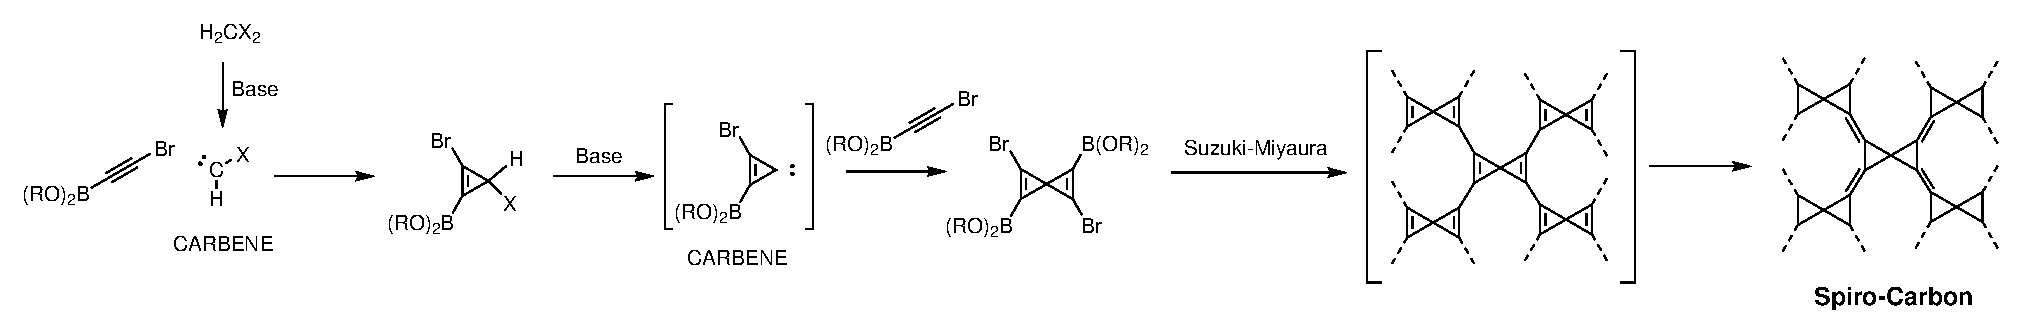
\includegraphics[width=1.\linewidth]{capitulos/fig/results1/synthesis_polyspiro1.eps}
		\caption{Possível rota sintética para a obtenção do Spiro-Carbon}
		\label{synthesis}
	\end{figure}


	\begin{figure}[ht]
		\centering
		\subfloat{
			\includegraphics[width=.4\linewidth]{capitulos/fig/IR}}
		\subfloat{
			\includegraphics[width=.4\linewidth]{capitulos/fig/RMN}}\\
		\subfloat{
			\includegraphics[width=.4\linewidth]{capitulos/fig/DRX}}
		\subfloat{
			\includegraphics[width=.4\linewidth]{capitulos/fig/UV-VIS}}
		\caption{Gráficos dos espectros calculados de (a) FTIR (Lorentziana com 10 cm$^{-1}$ de largura); (b) deslocamentos químicos isotrópicos de \textsuperscript{13}C RMN (Lorentziana com 1 ppm de largura); (c) Difratograma de raios-X; (d) Espectro de absorção UV-VIS (Lorentziana com 0.02 Ry de largura)}
		\label{charac}
	\end{figure}

	Na \autoref{charac} são apresentados os espectros simulados de FTIR, \textsuperscript{13}C RMN, difração de raios-X e absorção no UV-VIS para o Spiro-Carbon, na esperança de que sejam úteis no auxílio da caracterização de possíveis candidatos. O espectro de FTIR (\autoref{charac}-\textbf{a}) apresenta um pico principal em 918 cm\textsuperscript{-1} devido ao modo vibracional com simetria E\textsubscript{u} e dois picos menores em 527 e 1100 cm\textsuperscript{-1} devido aos modos  E\textsubscript{u} and A\textsubscript{2u}, respectivamente. O espectro de \textsuperscript{13}C RMN, mostrado na \autoref{charac}-b, apresenta dois deslocamentos químicos diferentes: 47.0 ppm para o átomo C1 e 133.6 ppm para o átomo C2. O espectro de difração de raios-X, apresentado na \autoref{charac}-c, calculado para comprimento de onda de 1.54059 \AA{} apresenta um pico principal em 18.5\textsuperscript{o} referente ao plano de Bragg (101) e picos menores em 29.8\textsuperscript{o} e 35.0\textsuperscript{o}, referentes aos planos (112) e (200), respectivamente.
	
	\subsection{Spiro-carbon como um material microporoso}
	
	\begin{figure}[ht]
		\centering
		\subfloat{
			\includegraphics[width=.4\linewidth]{capitulos/fig/h2_h}}\\
		\subfloat{
			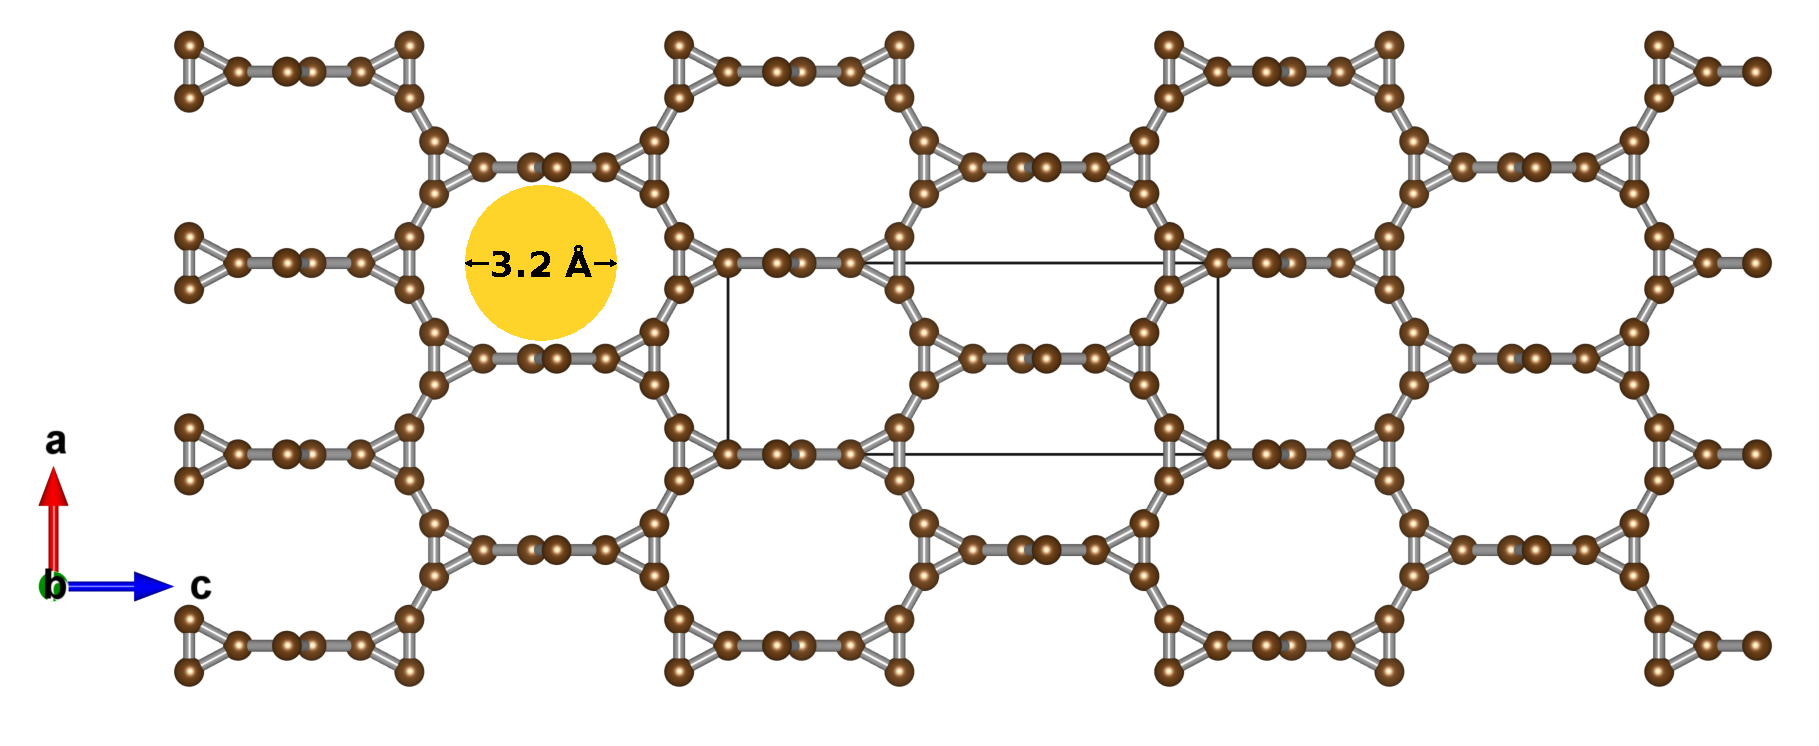
\includegraphics[width=0.8\linewidth]{capitulos/fig/pores.eps}}
		\caption{(a) Adsorção isotérmica de H\textsubscript{2}; (e) Representação da estrutura microporosa do Spiro-Carbon.}
		\label{charac_poros}
	\end{figure}

	Um aspecto que pode ser explorado nesse novo material proposto é sua estrutura porosa, representada na \autoref{charac_poros}-\textbf{b}. A máxima esfera que pode ser incluída dentro dos poros do Spiro-Carbon apresenta diâmetro de 3.21 \AA{}. A área de superfície geometricamente acessível para essa estrutura é de 2296 m\textsuperscript{2}/g. Sendo assim, esse material poderia potencialmente ser um adsorvente seletivo para gases, particularmente aqueles compostos por moléculas pequenas, como H\textsubscript{2} por exemplo. Para avaliar a viabilidade desta aplicação cálculos Monte Carlo Grand-Canônicos foram executados a fim de obter a capacidade de adsorção de H\textsubscript{2}, N\textsubscript{2} e CO\textsubscript{2}. Na \autoref{charac_poros}-\textbf{a} pode-se observar uma isoterma de adsorção de H\textsubscript{2} do tipo I(a), típica de sólidos microporosos. \cite{thommes2015physisorption} 
	
	A capacidade adsortiva de H\textsubscript{2} à 77K em 1 bar (100 kPa) calculada foi de 373 cm\textsuperscript{3}/g, aproximadamente 3.35\% em peso. Esse valor é consideravelmente alto, o que inclui o Spiro-Carbon na classe de materiais microporosos com excepcional capacidade de adsorção de H\textsubscript{2}.  \cite{blankenship2017cigarette, wong2006exceptional} Cálculos similares para a adsorção de moléculas maiores, como N\textsubscript{2} e CO\textsubscript{2} revelaram que essas moléculas não caberiam dentro dos poros. Dessa forma, o Spiro-Carbon pode ser considerado um adsorvente seletivo e exclusivo para H\textsubscript{2}.
	
	\subsection{Conclusões}
	
		Nesta seção um novo alótropo de carbono nomeado Spiro-Carbon, que, na extensão de nosso conhecimento ainda não foi relatado na literatura, foi estudado por cálculos em nível DFT PBE-D3. Com base nos dados apresentados podemos concluir que esta estrutura é um mínimo na superfície de potencial, é mecanicamente estável e apresenta caráter eletrônico metálico peculiar. Ele também apresenta menor energia de formação que outras formas alotrópicas tridimensionais do carbono, como Y-, Y-II-, T-, e T-II-Carbon, e potencial aplicação como adsorvente seletivo para H$_2$.  
		
		Os resultados discutidos nesta seção resultaram na publicação do artigo:
		
		\begin{citacao}
			Oliveira, F.L., Capaz, R.B. and Esteves, P.M., \textit{Spiro-Carbon}: A metallic carbon allotrope predicted from first principles calculations. \textbf{Chem. Phys. Chem.}, v.21, n.1, p.59-64, 2020.
		\end{citacao}
		
\section{ABF-Carbon}
		
		Tomando com base o motivo estrutural explorado no alótropo de carbono da seção anterior, o motivo \textbf{\textit{spiro}}, podemos conceber uma miríade de outras estruturas. Poderíamos, por exemplo, utilizar a estratégia de inserir unidades de acetileno entre as unidades spiro, formando estruturas conjugadas com poros progressivamente maiores como explorado em \cite{costa2018n}. Por outro lado, é possível conectar o motivo estrutural diretamente a átomos de carbono \textit{sp\textsuperscript{3}}, formando estruturas porosas semelhantes ao Spiro-Carbon, porém sem a conjugação entre as ligações duplas, gerando um potencial alótropo de carbono 3D semi-condutor. Essa estrutura hipotética será explorada ao longo dessa próxima seção.
	
	\subsection{Estrutura}
	
				
		\begin{figure}[ht!]
			\centering
			\includegraphics[width=.9\linewidth]{capitulos/fig/results2/structure}
			\caption{Representação da célula unitária do ABF-Spiro vista na direção dos vetores a) \textbf{a}, b) \textbf{b}, c) \textbf{c}, d) representação de célula primitiva e e). Representação da estrutura atômica da célula unitária tetragonal para o ABF-Carbon, com os átomos não equivalentes destacados em cores diferentes.}
			\label{structure_homospiro}
		\end{figure}	
	
		Essa estrutura idealizada, que pode representada por uma rede 3D do tipo \textbf{abf} \footnote{http://rcsr.anu.edu.au/nets/abf\#} e por isso será nomeada como ABF-Carbon, apresenta 6 átomos em uma célula unitária primitiva tetragonal de corpo centrado, com grupo espacial $I\bar{4}m2$ (\#119) e grupo pontual $D_{2d}^{11}$. A geometria de equilíbrio obtida a partir da otimização completa da estrutura apresenta parâmetros de célula \textit{a} = \textit{b} = 3.811 \AA{}, \textit{c} = 8.726 \AA{} e $\alpha$ = $\beta$ = $\gamma$ = 90$^\circ$, apresentando densidade de 1.89 g/cm$^3$. A célula unitária primitiva e convencional resultante é apresentada na \autoref{structure_homospiro}.

		
		Baseado na simetria do grupo espacial desta estrutura os três átomos não equivalentes ocupam os sítios de Wyckoff 8i, 2a e 2d, como representado na \autoref{structure_homospiro}-e). O átomo \textbf{C1} (verde) ocupa o sítio 8i e apresenta coordenadas fracionárias (0.00000, 0.00000, 0.00000), \textbf{C2} (amarelo) ocupa o sítio 2a e apresenta coordenadas (0.82651, 0.00000, 0.15266) e \textbf{C3} (azul) ocupa o sítio 2d apresentando coordenadas (0.00000, 0.50000, 0.75000). Baseado na estrutura otimizada é possível distinguir três diferentes tipos de ligação: \textit{i)} As ligações do átomo $sp^3$ da unidade \textit{spiro} com seus vizinhos (C1-C2) com comprimento iguais de 1.487 \AA{}; \textit{ii)} as ligações entre os átomos \textbf{C2} (C2=C2), com comprimento de 1.322 \AA{}, fechando o anel de 3 membros e formando a unidade spiro; \textit{iii)} as ligações das unidades \textit{spiro} com o átomo de carbono $sp^3$ (\textbf{C3}), com comprimento de 1.506 \AA, comprimento típico de ligação simples entre átomos de carbono.
		
		Os ângulos internos da unidade \textit{spiro} são de 52.8$^\circ$ (C2-C1-C2) e 63.6$^\circ$ (C1-C2-C2), valores iguais aos apresentados pelo análogo molecular spiropentadieno. Os ângulos das ligações do átomo de carbono \textbf{C3} apresentam um leve desvio do padrão para um tetraedro perfeito, de 109.5$^\circ$, apresentando valores de 111.4$^\circ$ e 108.5$^\circ$.     
		
		É possível observar que nessa estrutura que os comprimentos e ângulos das ligações na unidade \textit{spiro} se assemelham muito mais ao seu análogo molecular, o spiropentadieno, do que na estrutura do Spiro-Carbon. Isso se dá pelo fato de que, nessa estrutura, as unidades \textit{spiro} estão ligadas diretamente a átomos de carbono $sp^3$, o que impede que ocorra a conjugação entre as ligações duplas e fazendo que as ocorra uma localização maior das ligações duplas e simples. Isso nos permite antecipar que essa estrutura apresentará um caráter semi-condutor com \textit{band gap} relativamente grande, devido à dificuldade de interação entre os orbitais $\pi$. 
		
	\subsection{Estabilidade Relativa e Propriedades Mecânicas}
	
		Para investigar a estabilidade relativa desta estrutura, foi calculada a dispersão de fônons ao longo de um caminho entre pontos de alta simetria na primeira zona de Brillouin \cite{bradley2010mathematical}. Como pode ser observado na \autoref{ph_DOS-2}-\textbf{a)} não há a presença de nenhuma frequência imaginária, indicando que a estrutura do ABF-Carbon corresponde a um mínimo na superfície de potencial. 
	
		\begin{figure}[ht]
			\centering
			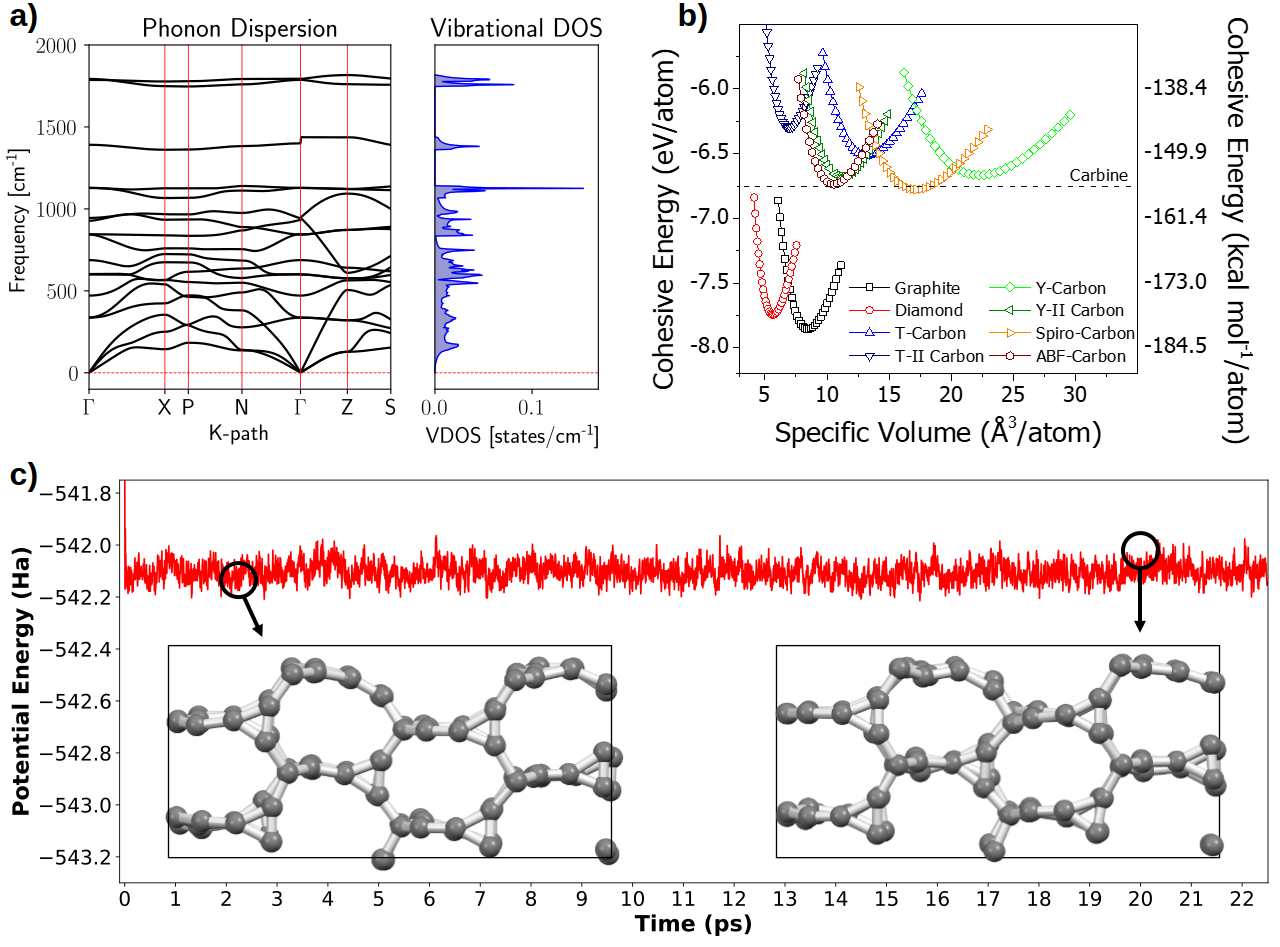
\includegraphics[width=1\linewidth]{capitulos/fig/results2/cohesive_abf-carbon}
			\caption{Gráfico da dispersão de fônons ao longo de alguns pontos de alta simetria na primeira zona de Brillouin e a correspondente densidade de estados vibracionais (VDOS) para o ABF-Carbon.}
			\label{ph_DOS-2}
		\end{figure}

		Para avaliar a estabilidade termodinâmica relativa do ABF-Carbon, a \autoref{ph_DOS-2}-\textbf{b)} mostra a variação da energia coesiva em função do volume (ambos por átomo) para diferentes alótropos de carbono. Como esperado, a curva $E_c(V)$ para o ABF-Carbon apresenta claramente um mínimo correspondente ao estado meta-estável desta estrutura. Assim como o Spiro-Carbon, esta estrutura se mostrou mais estável do que outros alótropos de carbono tridimensionais  como  1-diamantino/Y-Carbon \cite{costa2018n,li2014modulated} por aproximadamente 1.55 kcal/mol (0.07 eV) por átomo e o T-Carbon \cite{sheng2011t} por aproximadamente 5.1 kcal/mol (0.22 eV), como mostrado na \autoref{energy-abf}. 
		
		Curiosamente o ABF-Carbon apresentou energia coesiva cerca de 1.0 kcal/mol (0.05 eV) menor do que o Spiro-Carbon. Em geral, é esperado que uma estrutura que apresente mais átomos de carbono com hibridização $sp^3$ apresente maior estabilidade, entretanto, o ABF-Carbon mesmo apresentando uma razão de átomos $sp^2$/$sp^3$ de 2/1, valor menor do que o apresentado pelo Spiro-Carbon de 4/1, apresenta menor energia de formação. Este fenômeno é bastante incomum, e pode ter uma relação direta com o fato de o grafite possuir energia coesiva maior do que o diamante. Talvez a deslocalização gerada pela formação de ligações $\pi$ conjugadas, como acontece no grafite e no Spiro-Carbon, seja um fator estabilizante maior do que a sobreposição frontal dos orbitais gerada pela formação das ligações $\sigma$ em estruturas como a do diamante e do ABF-Carbon. Esse fenômeno ainda não apresenta uma resposta conclusiva na literatura, e pesquisas mais aprofundadas devem ser feitas para tentar explicar esse resultado contra-intuitivo. 
		
		\begin{table*}[ht]
			\centering
			\renewcommand{\arraystretch}{1.1}
			\caption{Módulo das energias relativa e coesiva por átomo para o ABF-Carbon comparado com diferentes alótropos de carbono.}
			\label{energy-abf}
			\begin{tabular}{lcccc}
				\hline
				\hline
				\multicolumn{1}{c}{\multirow{2}{*}{Estrutura}} & \multicolumn{2}{c}{Energia Relativa} & \multicolumn{2}{c}{Energia Coesiva}                             \\ \cline{2-5} 
				\multicolumn{1}{c}{}                           & \multicolumn{1}{l}{eV/átomo} & \multicolumn{1}{l}{kcal/mol/átomo} & \multicolumn{1}{l}{eV/átomo} & \multicolumn{1}{l}{kcal/mol/átomo} \\ \hline
				Grafite      & 0.000  & 0.000  & 7.856  & 181.16  \\
				Diamante     & 0.112  & 2.57   & 7.744  & 178.59  \\
				Spiro-Carbon & 1.079  & 24.88  & 6.777  & 156.29  \\
				Carbina      & 1.106  & 25.50  & 6.750  & 155.67  \\
				ABF-Carbon   & 1.121  & 25.86  & 6.735  & 155.30  \\
				Y Carbon     & 1.189  & 27.41  & 6.667  & 153.75  \\
				Y-II Carbon  & 1.177  & 27.15  & 6.679  & 154.01  \\
				T Carbon     & 1.342  & 30.94  & 6.514  & 150.22  \\
				T-II Carbon  & 1.554  & 35.84  & 6.302  & 145.32  \\ \hline \hline
			\end{tabular}
		\end{table*}
		
		
		Avaliando as seis constantes elásticas ($\textbf{C}_{ij}$ em GPa) calculadas, apresentadas na \autoref{elastic_ABF}, é fácil ver que as condições necessárias e suficientes que devem ser satisfeitas, baseadas nos critérios de estabilidade de Born \cite{born1940stability}, para garantir a estabilidade mecânica para uma rede tetragonal são satisfeitos pelo ABF-Carbon, indicando que essa nova estrutura proposta é mecanicamente estável. 
		
		\begin{table}[ht]
			\centering
			\renewcommand{\arraystretch}{1.1}
			\caption{Constantes elásticas ($\textbf{C}_{ij}$), módulo Bulk (\textbf{B}), shear (\textbf{G}) e Young (\textbf{E}) (em GPa), razão de Poisson ($\nu$) e dureza de Vicker ($H_v$) calculados para o Diamante, Spiro-Carbon e ABF-Carbon}
			\label{elastic_ABF}
			\begin{tabular}{lccc}
				\hline \hline
				& Diamante & Spiro-Carbon & ABF-Carbon \\\hline
				\textbf{C\textsubscript{11}} & 1106.43   & 277.76   & 481.72  \\
				\textbf{C\textsubscript{33}} & 1106.43   & 308.54   & 560.51  \\
				\textbf{C\textsubscript{44}} &  591.34   & 75.04    & 120.03  \\
				\textbf{C\textsubscript{66}} &  591.34   & 3.61     &  38.09  \\
				\textbf{C\textsubscript{12}} &  153.08   & 3.36     &  10.04  \\
				\textbf{C\textsubscript{13}} &  153.08   & 68.88    &  90.13  \\
				\textbf{B}                   &  470.86   & 123.73   & 209.37  \\
				\textbf{G}                   &  542.45   & 47.79    & 120.30  \\
				\textbf{E}                   & 1175.83   & 121.98   & 301.40  \\
				\textbf{$\nu$}               &   0.084   & 0.276    & 0.253   \\
				\textbf{$H_v$}               &   90.87   & 4.37    & 14.23   \\
				\hline \hline
			\end{tabular}
			\noindent
		\end{table}
		
		
		
		\begin{figure*}[!ht]
			\centering
			\includegraphics[width=1\linewidth]{capitulos/fig/results2/elastic_abf}
			\caption{Dependência espacial do (a) módulo de Young; (b) compressibilidade linear; (c) módulo Shear e (d) razão de Poisson para o ABF-Carbon.}
			\label{plot_elastic_ABF}
		\end{figure*}
		
		A \autoref{plot_elastic_ABF} mostra os gráficos da dependência espacial nos planos \textbf{xy}, \textbf{xz} e \textbf{yz} para os módulos de Young (\textbf{E}) e shear (\textbf{G}), compressibilidade linear  ($\beta$) e razão de Poisson ($\nu$), calculadas a partir das constantes elásticas apresentadas na \autoref{elastic_ABF}. É possível notar uma anisotropia do módulo de Young e módulo shear semelhante à apresentada pelo Spiro-Carbon, porém com menor intensidade. Esse resultado pode ser associado com a presença do átomo de carbono $sp^3$ conectando as unidade spiro na formação da estrutura estendida, conferindo maior rigidez e menor anisotropia a esse material. De fato, a anisotropia do módulo de Young é de A\textsubscript{E} = 4.03 e do módulo de cisalhamento é de A\textsubscript{G} = 5.55, valores muito menores que o para o Spiro-Carbon que são de 19.58 e 29.98, respectivamente.
			
		Utilizando o modelo empírico de \citeauthor{chen2011modeling} para o cálculo  da dureza de Vicker, o valor obtido para o ABF-Carbon é de 14.23 GPa (1452 HV). Esse valor é 3.25 vezes maior do que o apresentado pelo Spiro-Carbon, confiando que a adição dos átomos de carbono sp$^3$ na estrutura aumentam sua rigidez e dureza.
		%1 HV = 0.009807 GPa
		
	\subsection{Propriedades Eletrônicas}
		
		A estrutura do ABF-Carbon, ao contrário do Spiro-Carbon, apresenta ligações duplas localizadas nas unidades \textit{spiro} sem a possibilidade de conjugação, fazendo com que esse material possa apresentar um caráter semi-condutor. O \textit{gap} HOMO-LUMO calculado para a molécula do spiropentadieno é de 3.92 eV e 5.22 eV quando calculado como os funcionais PBE e HSE, respectivamente.\footnote{Ver Apêndice \autoref{chap:spiropentadiene} para mais detalhes} O diagrama de bandas calculado em nível PBE, apresentado na \autoref{band_ABF}, confirma o caráter semi-condutor com \textit{band gap} direto da estrutura. Além disso, é possível observar que a densidade de estados próxima ao nível de Fermi é formada unicamente pelos orbitais $2p$ ($2p_x$, $2p_y$ e $2p_z$). O \textit{band gap} direto calculado nesse nível é de 1.35 eV e 2.39 eV com o funcional HSE, indicando que essa estrutura apresenta um grande potencial para aplicações em optoeletrônica e fotocatálise.
		
		
		\begin{figure}[!ht]
			\centering
			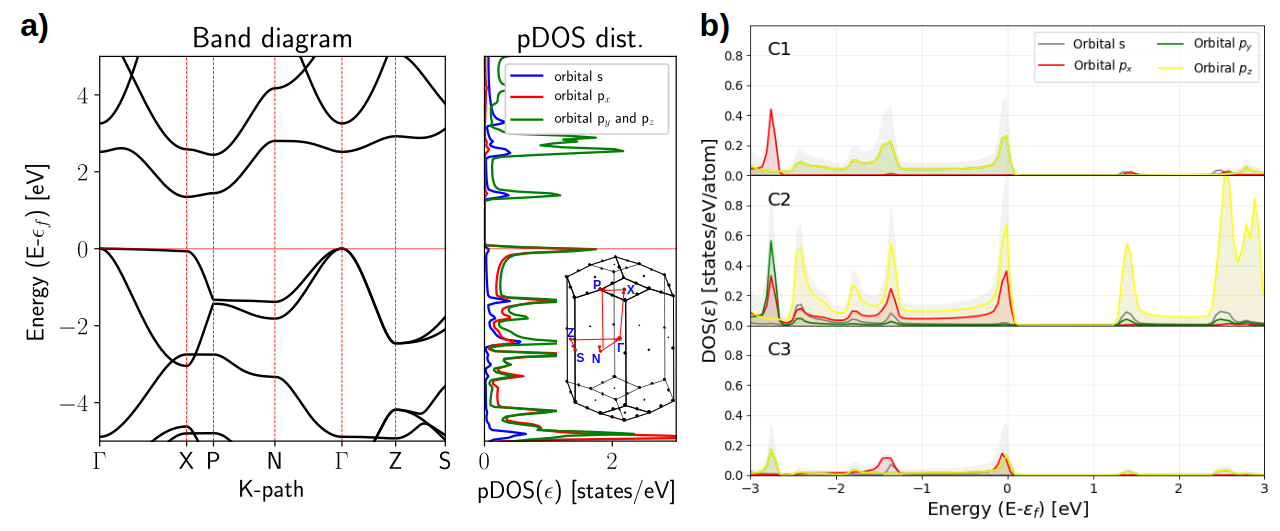
\includegraphics[width=.7\linewidth]{capitulos/fig/results2/band_structure}
			\caption{Dispersão de energia das bandas ao longo dos principais pontos de alta simetria na primeira zona de Brillouin (direita) e densidade de estados projetada nos orbitais (esquerda) para o ABF-Carbon. A energia de Fermi ($\epsilon_f$) foi ajustada para 0.}
			\label{band_ABF}
		\end{figure}
		
	\subsection{Caracterização}
		
		Na \autoref{carac_abf} são apresentados os espectros simulados de FTIR, \textsuperscript{13}C RMN e difração de raios-x e espectro de absorção no UV-VIS para o ABF-Carbon, na esperança de que sejam úteis no auxílio da caracterização de possíveis candidatos. O espectro de FTIR (\autoref{carac_abf}-\textbf{a}) apresenta um pico principal em 1391 cm\textsuperscript{-1} devido ao modo vibracional com simetria B\textsubscript{2} e um pico  em 927 cm\textsuperscript{-1} devido a outro modo B\textsubscript{2}. O espectro de \textsuperscript{13}C RMN, mostrado na \autoref{carac_abf}-\textbf{b}, apresenta três deslocamentos químicos diferentes: 128.5 ppm para o átomo C1, 44.2 ppm para o átomo C2 e 39.2 para o átomo C3. O espectro de difração de raios-X, apresentado na \autoref{carac_abf}-\textbf{c}, calculado para comprimento de onda de 1.54059 \AA{} apresenta um pico principal em 25.5\textsuperscript{o} referente ao plano de Bragg (101) e picos menores em 20.3\textsuperscript{o} e 33.2\textsuperscript{o}, referentes aos planos (002) e (110), respectivamente. O espectro de absorção na região do UV-VIS apresenta bandas em 280, 320, 480 e 960 nm, indicando grande potencial para aplicações que dependam de absorção de luz em regiões no espectro visível e próximas. Essa estrutura não apresentam poros com tamanho suficiente para ser acessível a nenhum átomo ou molécula. 
	
		\begin{figure}[!ht]
			\centering
			\includegraphics[width=1\linewidth]{capitulos/fig/results2/carac_ABF}
			\caption{Gráficos dos espectros calculados de (a) FTIR (Lorentziana com 10 cm$^{-1}$ de largura); (b) deslocamentos químicos isotrópicos de \textsuperscript{13}C RMN (Lorentziana com 1 ppm de largura); (c) Difratograma de raios-X; (d) Espectro de absorção no UV-VIS (Lorentziana com 0.02 Ry de largura).}
			\label{carac_abf}
		\end{figure}

	\subsection{Conclusões}
	
		Nesta seção foi apresentado um novo alótropo de carbono, denominado ABF-Carbon, formado pela conexão de unidades \textit{spiro} por átomos de carbono sp\textsuperscript{3}. Com base nos resultados apresentados é possível concluir que essa nova estrutura é estável, pois não apresenta frequências negativas na dispersão de fônons e sua matriz elástica satisfaz os critérios de estabilidade de Born. Diferentemente do Spiro-Carbon, essa estrutura apresenta um caráter semicondutor, com \textit{band gap} de 2.4 eV. Além disso, ela apresenta menor energia de formação que outras estruturas alotrópicas tridimensionais, encorajando possíveis tentativas de síntese.

\chapter{Gerando novos alótropos}
\label{alotropos_carbina}
	
	Na \autoref{sec:spiro} deste trabalho foi apresentado a estrutura do Spiro-Carbon e um dos aspectos mais marcantes é sua semelhança com cadeias de \textit{trans-cisoide}-(poli)acetileno conectadas por átomos de carbono $sp^3$, a origem de seu caráter metálico. Apesar de não ser um conceito prático, afinal polimerizar cadeias de (poli)acetileno para formar a estrutura cristalina do Spiro-Carbon pode ser um desafio sintético insuperável, utilizar uma molécula, ou motivo estrutural derivado de uma, como bloco de construção pode ser uma estratégia promissora para a idealização de novos alótropos de carbono.
	
	De fato, alguns trabalhos recentes na literatura mostram que utilizar alótropos já existentes como ponto de partida para novas estruturas pode ser uma ótima estratégia. \citeauthor{hu2013compressed} em \citeyear{hu2013compressed} mostrou que nanotubos de carbono comprimidos podem reorganizar suas ligações e formar novas estruturas. \citeauthor{fedik2020can} em \citeyear{fedik2020can} mostrou que o cyclo[18]carbon pode ser entrelaçado, como anéis em uma corrente, para formar catenanos de carbono. 
			
	\begin{figure}[!ht]
		\centering
		\includegraphics[width=.7\linewidth]{capitulos/fig/results3/carbina}
		\caption{Possíveis distorções da cadeia do carbino.}
		\label{carbina}
	\end{figure}

	Se olharmos para os modos normais de vibração do carbino, como apresentado na \autoref{carbina}, é possível perceber que dependendo de como esse modos se acoplam podem ser geradas duas formas muito parecidas com as diferentes configurações da cadeia de (poli)acetileno: um carbino em forma \textit{armchair} \textbf{(a)}, semelhante ao \textit{cis}-(poli)acetileno, e uma em forma \textit{zigue-zague} \textbf{(b)}, semelhante ao \textit{trans}-(poli)acetileno.
	
	Dessa forma, é possível pensar na formação de alótropos de carbono como o grafeno, ou até mesmo o Spiro-Carbon, a partir de cadeias do carbino distorcidas na direção de um de seus modos normais de vibração. Se a cadeia for distorcida na forma \textit{zigue-zague} e forem aproximadas de maneira paralela poderia ocorrer a quebra de uma ligação $\pi$ e consequente formação de ligações entre as cadeias, gerando assim a estrutura do grafeno. Por outro lado, se as cadeias fossem distorcidas na forma \textit{armchair} e fossem aproximadas de um átomo de carbono de maneira perpendicular, poderia ocorrer a formação da estrutura do Spiro-Carbon. É importante ressaltar que esse método não é uma proposta de mecanismo de síntese, mas sim puramente um exercício mental para desenvolver uma lógica de construção de novas estruturas. 
	
	A partir dessa metodologia, o grafeno e o Spiro-Carbon não são as únicas estruturas que podem ser geradas. Podemos conectar as cadeias distorcidas na forma zigue-zague não paralelamente, como é feito para gerar o grafeno, mas sim perpendicularmente e obter a estrutura proposta por \citeauthor{hoffmann1983hypothetical} em \citeyear{hoffmann1983hypothetical}. Podemos conectar as cadeias do carbino não por apenas um átomo, mas por dois ou mais átomos de carbono gerando assim uma miríade de estruturas, como representado na \autoref{alotropos}. 
	
	\begin{figure}[!ht]
		\centering
		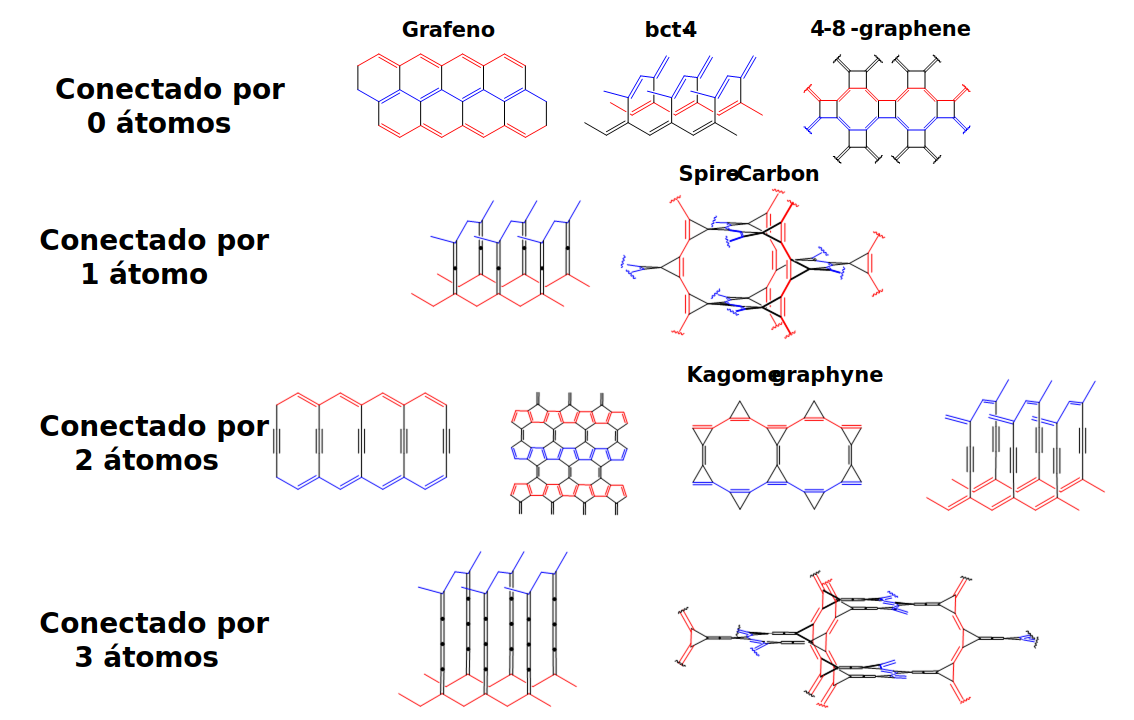
\includegraphics[width=1.\linewidth]{capitulos/fig/results3/alotropos}
		\caption{Diferentes alótropos que podem ser gerados a partir das diferentes formas de conectar o carbino.}
		\label{alotropos}
	\end{figure}

	\section{Conectando as cadeias diretamente}
		
		Seguindo a lógica de construção proposta, podemos gerar três estruturas diferentes conectando as cadeias diretamente. Utilizando a cadeia de carbino distorcida na forma \textit{zigue-zague} pode-se gerar a estrutura do grafeno (\autoref{0atomos}-\textbf{a}), se conectadas de maneira paralela, e a do bct-4 (\autoref{0atomos}-\textbf{b}), explorada por \citeauthor{hoffmann1983hypothetical}, se conectadas de maneira perpendicular. Utilizando a cadeia deformada na forma \textit{armchair} conectada diretamente de maneira paralela pode-se obter a estrutura (4,8)-carbon (\autoref{0atomos}-\textbf{c}), explorada por \citeauthor{nisar2012semiconducting}. Não é possível formar uma estrutura estável com a forma \textit{armchair} conectada perpendicularmente, pois dessa forma a distância entre dois átomos de cadeias adjacentes seria próxima do comprimento de uma ligação simples ($\approx$1.5 \AA{}). 
		
		A \autoref{0atomos} apresenta os cálculos do diagrama de bandas e dispersão de fônons para as três possíveis estruturas. É possível observar que nos três casos elas apresentam interseção entre as bandas de valência e condução, mostrando o caráter metálico já conhecido para essas estruturas. Uma característica que não é apresentada na literatura é a dispersão de fônons para o bct-4 (\autoref{0atomos}-\textbf{b}) e o (4,8)-carbon (\autoref{0atomos}-\textbf{c}). Os resultados para ambas as estruturas mostram uma grande incidência de modos vibracionais imaginários, indicando que nenhuma das estruturas é estável. De fato, no artigo original do bct-4 carbon os autores comentam que essa estrutura poderia apresentar uma espécie de "tensão $\pi$", devido à proximidade entre os orbitais $\pi$ na vizinhança de cada cadeia. Esse fator pode ser responsável pelas frequências vibracionais imaginárias apresentadas em \textbf{N}.
		
		\begin{figure}[!ht]
			\centering
			\includegraphics[width=1.\linewidth]{capitulos/fig/results3/0atoms}
			\caption{Diferentes alótropos que podem ser gerados a partir do carbino conectada diretamente.}
			\label{0atomos}
		\end{figure}
		
	\section{Conectando as cadeias por um átomo}
		
		Conectando as cadeias por um átomo pode-se gerar duas estruturas diferentes, sendo ambas tridimensionais. A primeira estrutura, derivada do carbino \textit{zigue-zague}, apresenta uma geometria parecida com a do bct-4, mas com as cadeias conectadas por duas ligações duplas cumulências (\autoref{1atomos}-\textbf{a}). A segunda é derivada do carbino \textit{armchair}, e já foi explorada na \autoref{sec:spiro} tendo sido denominada Spiro-Carbon (\autoref{1atomos}-\textbf{b}). Nenhuma das duas estruturas haviam sido relatadas na literatura anteriormente a esse trabalho. 
		
		\begin{figure}[!ht]
			\centering
			\includegraphics[width=1\linewidth]{capitulos/fig/results3/1atoms}
			\caption{Diferentes alótropos que podem ser gerados a partir do carbino conectada por um átomo de carbono.}
			\label{1atomos}
		\end{figure}
	
		Nenhuma das duas apresentaram frequências imaginárias na dispersão de fônons, indicando que as estruturas são um mínimo na superfície de energia potencial. Além disso, ambas as estruturas apresentam caráter eletrônico metálico com grande densidade de estados próximo ao nível de Fermi, uma consequência do caráter \textit{quasi}-unidimensional da cadeia do carbino.  
			
		
	\section{Conectando as cadeias por dois átomo ou mais átomos}
		
		Conectando as cadeias por dois átomos podemos gerar pelo menos quatro estruturas diferentes. Essa estratégia pode ser comparada a adicionar uma unidade acetilênica (-C$\equiv$C-) entre as cadeias do carbino distorcida, entretanto esses átomos têm a liberdade de apresentar ligações acetilênicas (ligando-se entre sí por ligações triplas e com seus vizinhos por ligações simples) ou ligações cumulênicas (formando uma sequência de três ligações duplas com orbitais $\pi$ perpendiculares). Das quatro estruturas possíveis, três são bidimensionais e somente uma tridimensional.   
		
		\begin{figure}[!ht]
			\centering
			\includegraphics[width=1\linewidth]{capitulos/fig/results3/2atoms}
			\caption{Diferentes alótropos que podem ser gerados conectando cadeias do carbino por dois átomos de carbono.}
			\label{2atomos}
		\end{figure}	
		
		Ao tentar conectar as cadeias por três ou mais átomos, é possível notar que a estrutura geral passa a seguir o mesmo padrão, porém agora com mais átomos entre as cadeias principais. Por exemplo, ao conectar o carbino \textit{armchair} por três átomos o motivo estrutural semelhante ao \textit{Spiro-Carbon} aparece, mas agora os anéis de três membros estão separados por um átomo de carbono e não mais ligados diretamente. O mesmo acontece com as cadeias \textit{zigue-zague} conectadas por três átomos, estruturalmente ela fica muito parecida com a conectada por apenas um átomo porém agora as cadeias do carbino estão mais espaçadas. 
		
		Por fim é importante ressaltar que o conceito geral de gerar novos alótropos segundo as direções das distorções provenientes dos modos normais de vibração não está limitado ao carbino. Podemos pensar em estruturas 3D, como o diamante ou o Lonsdaleite, como sendo formado por distorções seguindo os modos normais de vibração do grafeno, por exemplo. Seguindo essa mesma lógica, outros materiais 2D podem ser distorcidos e conectados para gerar novas estruturas tridimensionais. Isso abre intrigantes e excitantes perspectivas para pesquisas futuras, mostrando como ainda somente arranhamos a superfície de todo o potencial estrutural que um único tipo de átomo pode gerar. 
	
		
	\section{Conclusões}
		
		Neste capítulo foi explorado o conceito de obtenção de novos alótropos a partir de um alótropo já conhecido, o carbino. Seguindo a distorção de cadeia na direção de um de seus modos normais de vibração e combinando as cadeias de maneira paralela ou perpendicular é possível obter a estrutura de alótropos já conhecidos como o grafeno e o bct-4 carbon. Adicionando um ou mais átomos entre as cadeias é possível conceber uma variedade de novas estruturas, com propriedades eletrônicas completamente diferentes. 
		
		Esse conceito abre espaço para novas pesquisas futuras, utilizando não somente o carbino como "bloco de construção" para novos alótropos, mas também outras estruturas como o grafeno e nanotubos de carbono. Essa estratégia permite a criação de um espaço amostral de possíveis estruturas de maneira simples e objetiva, facilitando a busca pelas estruturas mais estáveis e/ou que apresentem propriedades especiais, e assim incentivando esforços experimentais para sintetizar alguns candidatos. 



% ----------------------------------------------------------
% Finaliza a parte no bookmark do PDF
% para que se inicie o bookmark na raiz
% e adiciona espaço de parte no Sumário
% ----------------------------------------------------------
\phantompart

% ---
% Conclusão
% ---
%% abtex2-modelo-include-comandos.tex, v-1.9.6 laurocesar
%% Copyright 2012-2016 by abnTeX2 group at http://www.abntex.net.br/ 
%%
%% This work may be distributed and/or modified under the
%% conditions of the LaTeX Project Public License, either version 1.3
%% of this license or (at your option) any later version.
%% The latest version of this license is in
%%   http://www.latex-project.org/lppl.txt
%% and version 1.3 or later is part of all distributions of LaTeX
%% version 2005/12/01 or later.
%%
%% This work has the LPPL maintenance status `maintained'.
%% 
%% The Current Maintainer of this work is the abnTeX2 team, led
%% by Lauro César Araujo. Further information are available on 
%% http://www.abntex.net.br/
%%
%% This work consists of the files abntex2-modelo-include-comandos.tex
%% and abntex2-modelo-img-marca.pdf
%%

% ---
% Este capítulo, utilizado por diferentes exemplos do abnTeX2, ilustra o uso de
% comandos do abnTeX2 e de LaTeX.
% ---

\chapter{Conclusão}
\label{conclusao}
	
	Com base nos resultados apresentados ao longo desta dissertação, é possível retomar as perguntas levantadas na seção de objetivos e apresentar uma resposta.
	
	\begin{enumerate}
		


		\item[$1^{\circ}$:] \textbf{É possível utilizar métodos DFT para predizer a estrutura e propriedades de diferentes alótropos de carbono?}
			
			Sim. Os resultados apresentados no \autoref{calculos_exp} permitem afirmar que os cálculos de estrutura eletrônica em nível DFT apresentam um bom resultado na predição da estrutura e propriedades, como \textit{band gap} e módulo Bulk por exemplo, dos alótropos de carbono que se têm dados experimentais para serem comparados. Os funcionais de troca-correlação avaliados apresentaram diferentes desempenhos, tendo o funcional PBE sido o que apresentou os resultados mais consistentes com os dados experimentais. Além disso, para sistemas cujas interações intermoleculares possuem um papel estrutural chave, como no grafite, uma correção de energia dispersiva deve ser adicionada aos funcionais GGA para garantir predições acuradas. A correção do tipo Grimme-D3 apresentou um melhor resultado, sendo portanto a indicada para cálculos futuros.
	
		\item[$2^{\circ}$:] \textbf{É possível propor novas estruturas alotrópicas metaestáveis para o carbono baseadas em motivos estruturais moleculares}
			
			Sim. No \autoref{chap:novos_alotropos} foram apresentadas duas novas formas alotrópicas para o carbono, denominadas Spiro-Carbon e ABF-Carbon, contendo o motivo estrutural derivado da molécula spiropentadieno. Os resultados apresentados mostram que ambas as estruturas correspondem a um mínimo na superfície de potencial, são mecanicamente estáveis e apresentam menor energia de formação que outros alótropos já obtidos experimentalmente, como o T-Carbon, ou ainda elusivos como o T-II-Carbon e Y-Carbon.
	
		\item[$3^{\circ}$:] \textbf{É possível utilizar uma forma alotrópica já existente, como por exemplo o carbino, como "\textit{blocos de construção}" para novos alótropos de carbono?}
		
			Sim. No \autoref{alotropos_carbina} foi mostrado que alótropos já conhecidos, como o grafeno e o bct-4, podem ser vistos como cadeias distorcidas do carbino conectadas de diferentes maneiras. Além disso, utilizando essa estratégia é possível construir um espaço amostral de diferentes estruturas possíveis o que pode levar à descoberta de diversas novas formas alotrópicas estáveis para o carbono.
		
	\end{enumerate}

% ---

% ----------------------------------------------------------
% ELEMENTOS PÓS-TEXTUAIS
% ----------------------------------------------------------
\postextual
% ----------------------------------------------------------

% ----------------------------------------------------------
% Referências bibliográficas
% ----------------------------------------------------------
\bibliography{bibliografia}

% ----------------------------------------------------------
% Glossário
% ----------------------------------------------------------
%
% Consulte o manual da classe abntex2 para orientações sobre o glossário.
%
%\glossary

% ----------------------------------------------------------
% Apêndices
% ----------------------------------------------------------

% ---
% Inicia os apêndices
% ---
\begin{apendicesenv}

% Imprime uma página indicando o início dos apêndices
\partapendices


% ----------------------------------------------------------
\chapter{}
\label{ap:conv}
% ----------------------------------------------------------
	
	\section{Energia de corte das funções de onda e grid de vetores $\vec{k}$}
		Para determinar os parâmetros básicos do cálculo, como a energia de corte para as ondas planas e a densidade do grid de vetores  $\vec{k}$, a \autoref{conv_diamante} mostra como a energia total, força total e pressão total variam em função desses dois parâmetros para o diamante. É possível observar que a convergência é atingida rapidamente, sendo que após 40 Ry como energia de corte e um grid de 6x6x6 não há mudança significativa em nenhuma das três propriedades. É possível observar também que o consumo de memória RAM e o tempo total de cálculo crescem aproximadamente linearmente com o aumento da energia de corte e de maneira quadrática com o aumento do grid de vetores $\vec{k}$.
	
		\begin{figure}[!h]
			\centering
			\subfloat{\includegraphics[width=.48\linewidth]{capitulos/fig/apendices/plot_Ecut_diamante}}
			\subfloat{\includegraphics[width=.48\linewidth]{capitulos/fig/apendices/plot_k_diamante}} 
			\caption{Convergência de diversas propriedades em função da energia de corte para as ondas planas (direita) e grid de vetores $\vec{k}$ (esquerda).}
			\label{conv_diamante}
		\end{figure}
		
		A \autoref{conv_spiro} apresenta os resultados para o mesmo teste com a estrutura do Spiro-Carbon. É possível observar um comportamento parecido como o diamante, com a convergência sendo atingida após 40 Ry e um grid de 6x6x6. Entretanto, como o cálculo de algumas propriedades como modos vibracionais e tensores de susceptibilidade magnética são mais sensíveis à pequenas variações na e energia, e portanto, podem apresentar uma convergência mais lenta para todos os cálculos foram utilizados 80 Ry como energia de corte para as funções de onda e um grid de vetores $\vec{k}$ de 12x12x12.
	
		\begin{figure}[!h]
			\centering
			\subfloat{\includegraphics[width=.48\linewidth]{capitulos/fig/apendices/plot_convE_Spiro}}
			\subfloat{\includegraphics[width=.48\linewidth]{capitulos/fig/apendices/plot_convK_Spiro}} 
			\caption{Convergência de diversas propriedades em função da energia de corte para as ondas planas (direita) e grid de vetores $\vec{k}$ (esquerda) para o Spiro-Carbon.}
			\label{conv_spiro}
		\end{figure}
	
	\section{Grid de vetores $\vec{\mathbf{q}}$ para dispersão de fônons}
		Outro parâmetro importante que deve ser avaliado é o grid de vetores $\vec{\mathbf{q}}$ utilizados para calcular a dispersão de fônons. Como a dispersão de fônons é calculada para os vetores compostos nesse grid que não equivalentes por simetria e esse tipo de cálculo é extremamente demorado e demanda considerável recurso computacional, é preciso utilizar o menor grid possível que apresente considerável confiabilidade. A \autoref{phgrid_diamante_q} apresenta a dispersão de fônons calculada com grids de vetores $\vec{\mathbf{q}}$ de 2x2x2 (Verde), 4x4x4 (Ciano), 6x6x6 (Marrom) e 8x8x8 (Púrpura). Como é possível observar, o grid de 4x4x4 já apresenta convergência satisfatória e, portanto, foi escolhido para todos os cálculos ao longo deste trabalho. 
		
		\begin{figure}[!h]
			\centering
			\includegraphics[width=1.\linewidth]{capitulos/fig/apendices/diamante_phdisp}
			\caption{Convergência da frequência dos modos vibracionais com o grid de $\vec{\mathbf{q}}$. Verde - 2x2x2, Ciano - 4x4x4, Marrom = 6x6x6 e Púrpura - 8x8x8.}
			\label{phgrid_diamante_q}
		\end{figure}


% ----------------------------------------------------------
	\section{Cálculos para a molécula Spiropentadieno} \label{chap:spiropentadiene}
% ----------------------------------------------------------
	\begin{figure}[!ht]
		\centering
		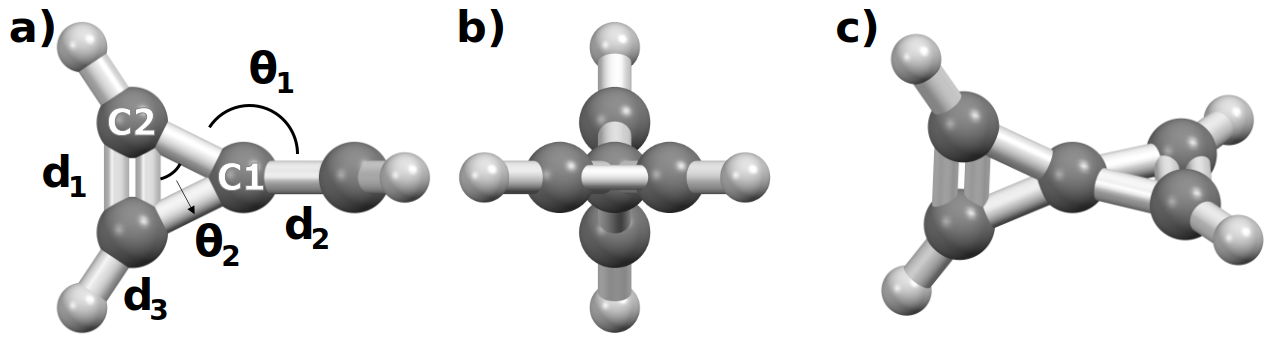
\includegraphics[width=1\linewidth]{capitulos/fig/apendices/spiropentadiene}
		\caption{Representação da estrutura da molécula spiropentadiene.}
		\label{strutura_spiropentadiene}
	\end{figure}
	
	

	\begin{table}[!ht]
		\centering
		\caption{Comparação entre valores calculados com diferentes funcionais para a molécula spiropentadiene.}
		\label{dados_spiropentadieno}
		\renewcommand{\arraystretch}{1.2}
		\fontfamily{lmss}\small\selectfont
		\begin{tabular}{l|cccccc}
			\hline\hline
						            &  $d_1$  & $d_2$ & $d_3$ & $\theta_1$ & $\theta_2$ & HOMO-LUMO.     \\
			  		 	            & (\AA{}) & (\AA{}) & (\AA{}) & ($^\circ$) & ($^\circ$)  & (eV)    \\ \hline
			HF/STO-3G \textsuperscript{\cite{kao1978ab}}  & 1.296   & 1.473   & 1.077   & 147.0      &    -     &  15.91  \\
			MP2/6-31+G(dp) \textsuperscript{\cite{shavitt1991ab}}  & 1.328   & 1.480   & 1.078   & 146.6      &    66.0     &  -  \\
			MP2/6-311++G** \textsuperscript{\cite{dodziuk2001theoretical}}  & 1.331   & 1.485   & 1.083   & 146.2      &    -     &  -  \\
			M062X/6-311+G(d,p)      & 1.311   & 1.477   & 1.080   & 150.2     &   63.6     &  3.94   \\
			GGA-PBE-D3/PW           & 1.319   & 1.482   & 1.087   & 150.1     &   63.6      & 3.92        \\
			HSE/PW                  &  -   & -   &         &     -       &      -       & 5.22        \\
			\hline\hline         
		\end{tabular}
	\end{table}
	
	
	Para comparação com as estruturas estendidas cálculos de referência para a molécula spiropentadieno (\autoref{strutura_spiropentadiene}) foram feitos e os resultados são apresentados na \autoref{dados_spiropentadieno}, comparados com outros resultados obtidos da literatura. 

% ----------------------------------------------------------
\section{Cálculos para (poli)acetileno} \label{chap:bands_poliacetileno}
% ----------------------------------------------------------
	
	A \autoref{bands_trans} apresenta o diagrama de bandas do \textit{trans}-(poli)acetileno de duas formas diferentes: \textit{a)} sem distorção de Peierls com ambas as ligações com o mesmo comprimento e \textit{band gap} igual a 0 eV e \textit{b)} com distorção de Peierls com duas ligações de comprimentos diferentes e apresentando \textit{band gap} de aproximadamente 0.3 eV.
	
	\begin{figure}[!ht]
		\centering
		\includegraphics[width=.65\linewidth]{capitulos/fig/apendices/trans_poliacetileno}
		\caption{Diagrama de bandas do a) \textit{trans}-(poli)acetileno e b) \textit{trans}-\textit{transoid}-(poli)acetileno.}
		\label{bands_trans}
	\end{figure}

	A \autoref{bands_cis} apresenta o diagrama de bandas do \textit{cis}-(poli)acetileno de três formas diferentes: \textit{a)} sem distorção de Peierls com ambas as ligações com o mesmo comprimento e \textit{band gap} igual a 0 eV, \textit{b)} com distorção de Peierls mas na forma do \textit{cis}-\textit{cisoid}-(poli)acetileno com \textit{band gap} igual a 0.8 eV e \textit{c)} com distorção de Peierls na forma da \textit{trans}-\textit{cisoid}-(poli)acetileno com band-gap igual a 0.3 eV

	\begin{figure}[!ht]
		\centering
		\includegraphics[width=1\linewidth]{capitulos/fig/apendices/cis_poliacetileno}
		\caption{Diagrama de bandas do a) \textit{cis}-(poli)acetileno, b) \textit{cis}-\textit{cisoid}-(poli)acetileno e c)\textit{trans}-\textit{cisoid}-(poli)acetileno.}
		\label{bands_cis}
	\end{figure}




\end{apendicesenv}
% ---


% ----------------------------------------------------------
% Anexos
% ----------------------------------------------------------

% ---
% Inicia os anexos
% ---
%\begin{anexosenv}

% Imprime uma página indicando o início dos anexos
%\partanexos

% ---
%\chapter{Artigos publicados}
% ---
%\include{capitulos/fig/apendices/cphc.201900966.pdf}
%\includepdf[pages=-,pagecommand={},width=\textwidth]{capitulos/fig/apendices/cphc201900966}
%\end{anexosenv}

%---------------------------------------------------------------------
% INDICE REMISSIVO
%---------------------------------------------------------------------
\phantompart
\printindex
%---------------------------------------------------------------------

\end{document}
